\documentclass[14pt]{beamer}

\usetheme{Madrid}

% Add frame numbers
\setbeamertemplate{page number in head/foot}[framenumber]

\usepackage{amsmath, amssymb}
\usepackage{tikz}
\usepackage{bm}
\usepackage{outlines}   % For multilevel lists using the outline environment
\usepackage{natbib}
\usepackage{subcaption}

\renewcommand*{\bibfont}{\scriptsize}

\newcommand{\CMA}{Causal Mediation Analysis}

\newcommand{\bE}{\mathbb{E}}
\newcommand{\bF}{\mathbb{F}}
\newcommand{\bG}{\mathbb{G}}

\newcommand{\GLMMs}{Mixed-Effects Models}

\title[]{Adaptive Pareto Smoothed Importance Sampling}
\author{William Ruth}
\institute[]{Université de Montréal}
\date{\vspace{-3cm}}
% \titlegraphic{
\includegraphics[width=2cm]{../Logos/CANSSI_Logo.png} \hspace{2cm} 
\includegraphics[width=4cm]{../Logos/Logo_UdeM-CMJN.jpg}}


\begin{document}

\begin{frame}
    \titlepage
\end{frame}

\begin{frame}{Who am I?}
    \begin{outline}
        \1 PhD SFU 2023
        \1 Postdoc UdeM (present) \newline

        \1 Computational Statistics
            \2 Simulation
            \2 Simulation-based inference
        \1 Infectious disease modelling
    \end{outline}
\end{frame}

\begin{frame}{Topics}
    \begin{outline}
        \1 Adaptive Pareto Smoothed Importance Sampling \newline
        \1 Multilevel Causal Mediation Analysis \newline
        \1 Modelling Tuberculosis in Foreign-Born Canadians
    \end{outline}
\end{frame}

\begin{frame}{Topics}
    \begin{outline}
        \1 \textbf{Adaptive Pareto Smoothed Importance Sampling} \newline
        \1 Multilevel Causal Mediation Analysis \newline
        \1 Modelling Tuberculosis in Foreign-Born Canadians
    \end{outline}
\end{frame}

\begin{frame}{Outline}
    \begin{outline}
        \1 Importance sampling \newline
        \1 Measuring performance \newline
        \1 Improving performance
            \2 Modifications
            \2 Optimization
    \end{outline}
\end{frame}


\begin{frame}{Importance Sampling}
    \begin{outline}
        \1 Need to compute an expected value
            \2 $\bE_F \varphi(X)$
        \1 Can't do the sum/integral \newline

        \1 Monte Carlo approximation
            \2 Simulating from $F$ might be hard
    \end{outline}
    \begin{equation*}
    \end{equation*}
\end{frame}

\begin{frame}{Importance Sampling}
    \begin{outline}
        \1 Introduce ``proposal distribution'', $G$:
    \end{outline}
    \begin{align*}
        \bE_F \varphi(X) &=  \bE_G \left[ \varphi(X) \cdot \frac{f(X)}{g(X)} \right] \\
        &=  \bE_G \left[ \varphi(X) \cdot w(X) \right]
    \end{align*}
    \begin{outline}
        \1 $G$ can be nearly anything*
            \2 *Some choices will be better than others
    \end{outline}
\end{frame}

\begin{frame}{Example: Mystery Target}
    \begin{outline}
        \1 $f$ unknown, but can be evaluated 
        \1 $\varphi(X) = X^2$ \newline

        \1 Try some proposals:
            \2 $G_1 \sim N(0, 2^2)$
            \2 $G_2 \sim N(0, 0.5^2)$ \newline
        \1 Use $M=1000$ samples from proposal
            \2 $\hat{\bE}_1 = 0.99$, $\hat{\text{SD}} = 1.97$
            \2 $\hat{\bE}_2 = 1.10$, $\hat{\text{SD}} = 2.32$
    \end{outline}    
\end{frame}

\begin{frame}{Example: Mystery Target}
    \centering
    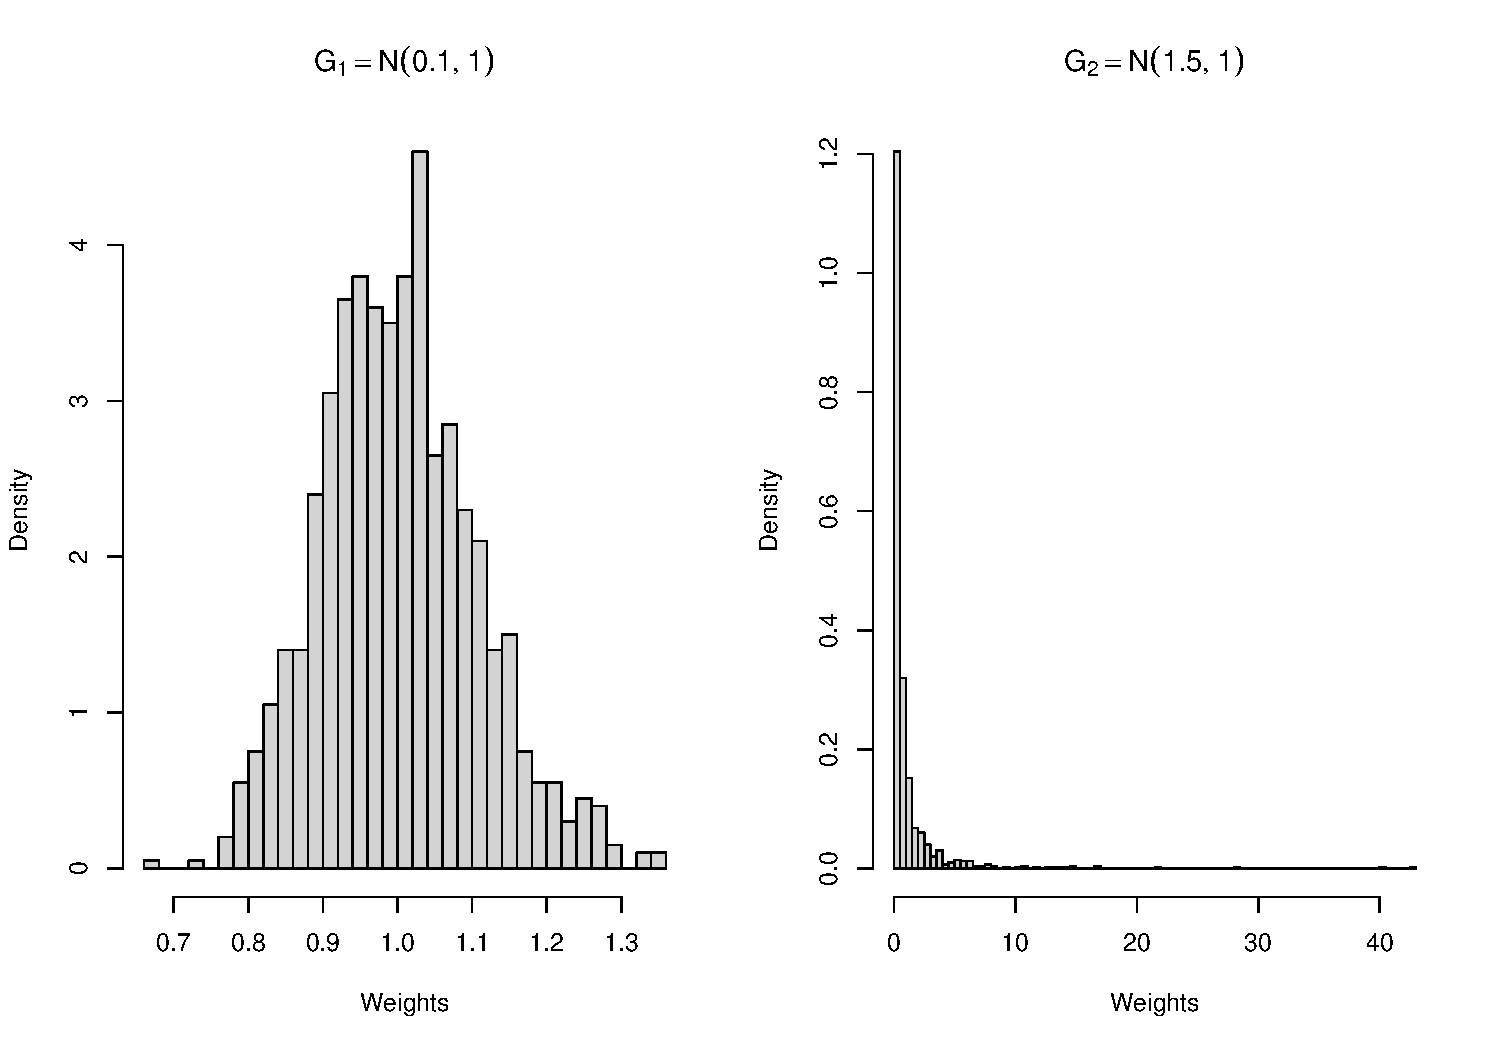
\includegraphics[height=0.9\textheight, width=0.9\textwidth, keepaspectratio]{Figures/Wt Hist.pdf}
\end{frame}

\begin{frame}{Importance Sampling}
    \begin{outline}
        \1 $G_1$ weights look fine
        \1 $G_2$ weights dominated by one large value \newline

        \1 We can make this difference precise
        \1 ``Effective Sample Size'':
    \end{outline}
    \begin{gather*}
        ESS = \frac{\left[\sum_i w(X_i)\right]^2}{\sum_i w(X_i)^2}
    \end{gather*}
\end{frame}

\begin{frame}{Example: Mystery Target}
    \centering
    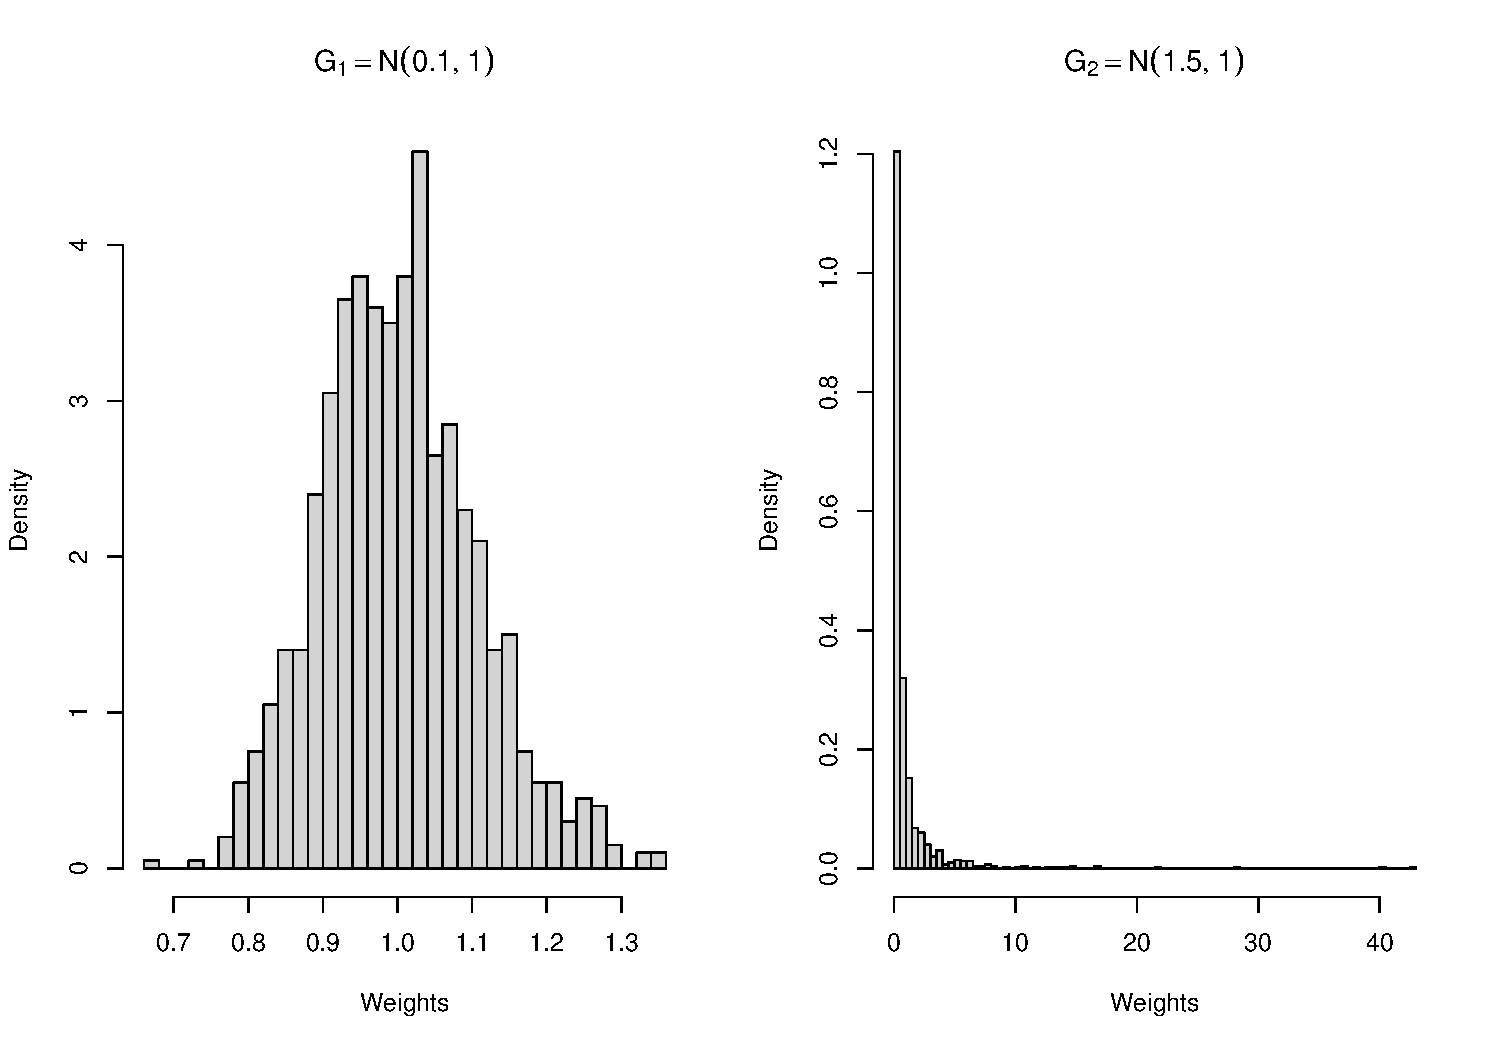
\includegraphics[height=0.7\textheight, width=0.9\textwidth, keepaspectratio]{Figures/Wt Hist.pdf} \newline
    \begin{outline}
        $ESS_1 \approx 662$ \hspace{2.5cm} $ESS_2 \approx 54$
    \end{outline}
\end{frame}

\begin{frame}{Importance Sampling}
    \begin{outline}
        \1 Problem: Low ESS $\rightarrow$ hard to estimate means \newline
        \1 But ESS is based on means
            \2 \citep{Cha18}
    \end{outline}
\end{frame}

% \begin{frame}{Importance Sampling}
%     \begin{outline}
%         \1 Consider $\varphi(X) = X$
%             \2 I.e. $\bE_F \varphi(X) = \bE_F(X)$ \newline
%         \1 $\hat{\bE} = \sum_i \frac{X_i w(X_i)}{M}$, $X_i \overset{\mathrm{iid}}{\sim} G$ \newline

%         \1 The variance of our estimator is \left( \sum_i w(X_i)^2 \right)
%     \end{outline}
% \end{frame}


\begin{frame}{Improving IS}
    \begin{outline}
        \1 Choose a good proposal \newline
        
        \1 Modify large weights        
            \2 Truncated IS
            \2 Pareto Smoothed IS
    \end{outline}
\end{frame}

\begin{frame}{Improving IS}
    \begin{outline}
        \1 Truncated Importance Sampling:
            \2 \citep{Ion08} \newline
    \end{outline}

    \setbeamertemplate{enumerate items}[default]
    \begin{enumerate}
        \item Choose a threshold
        \item Apply hard thresholding to any large weights \newline
    \end{enumerate}
    \begin{outline}
        \1 Still consistent for the target
    \end{outline}
\end{frame}

\begin{frame}{Example: Mystery Target}
    \centering
    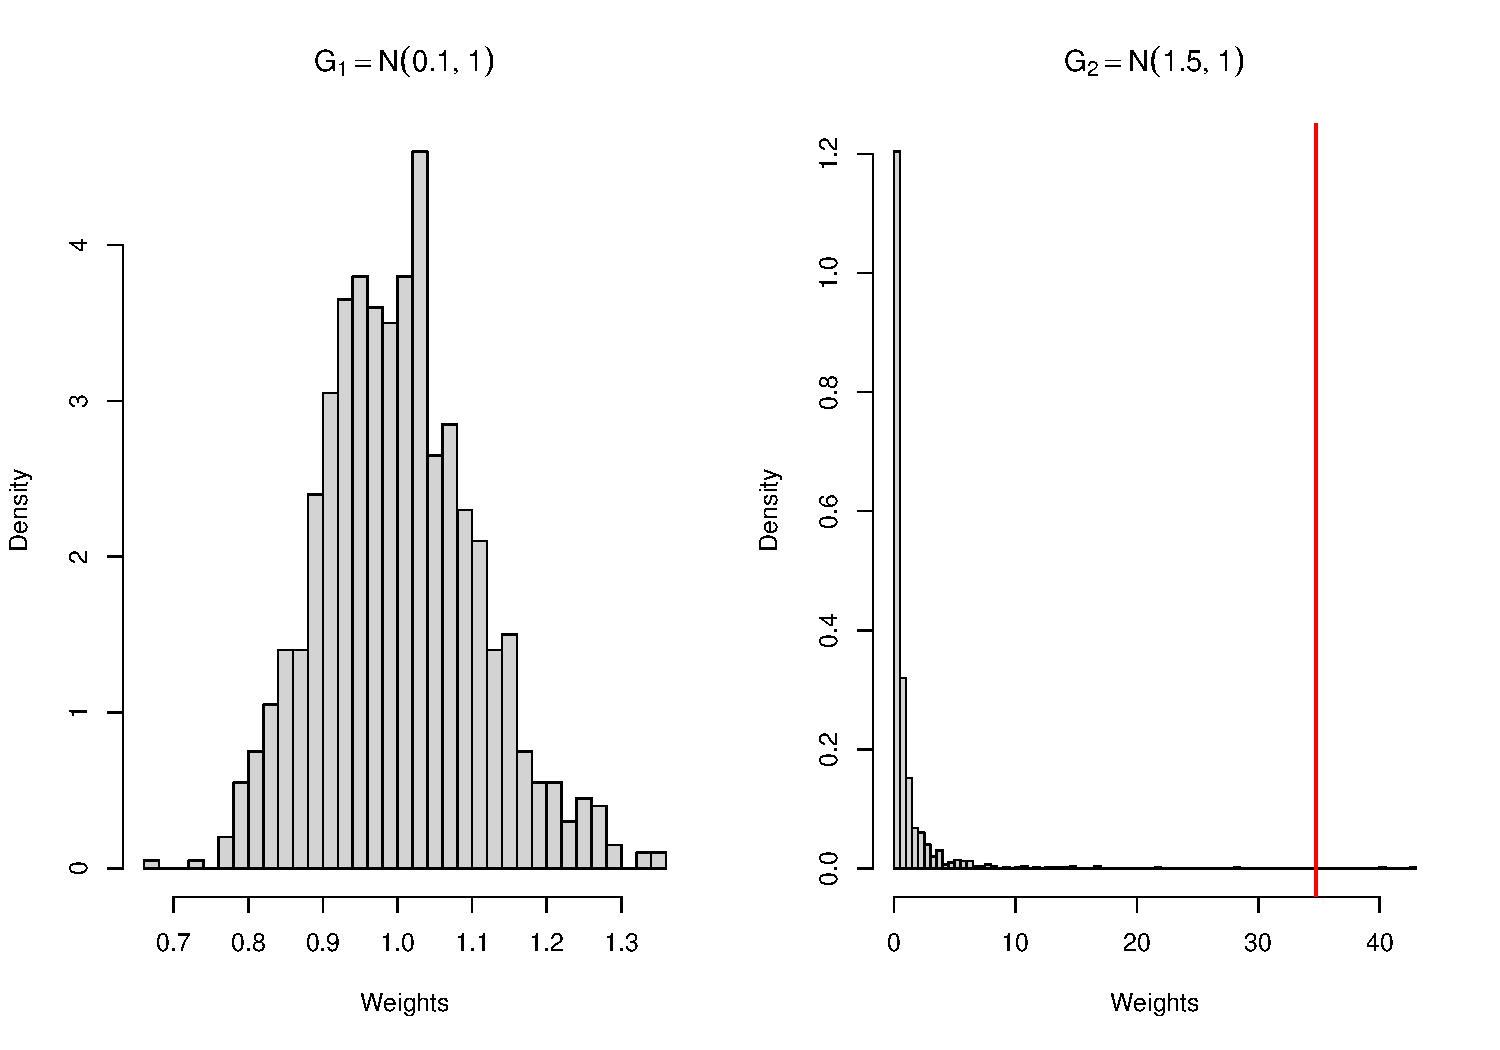
\includegraphics[height=0.9\textheight, width=0.9\textwidth, keepaspectratio]{Figures/Wt Hist - Thresh.pdf}
\end{frame}

% \begin{frame}{Example: Mystery Target}
%     \centering
%     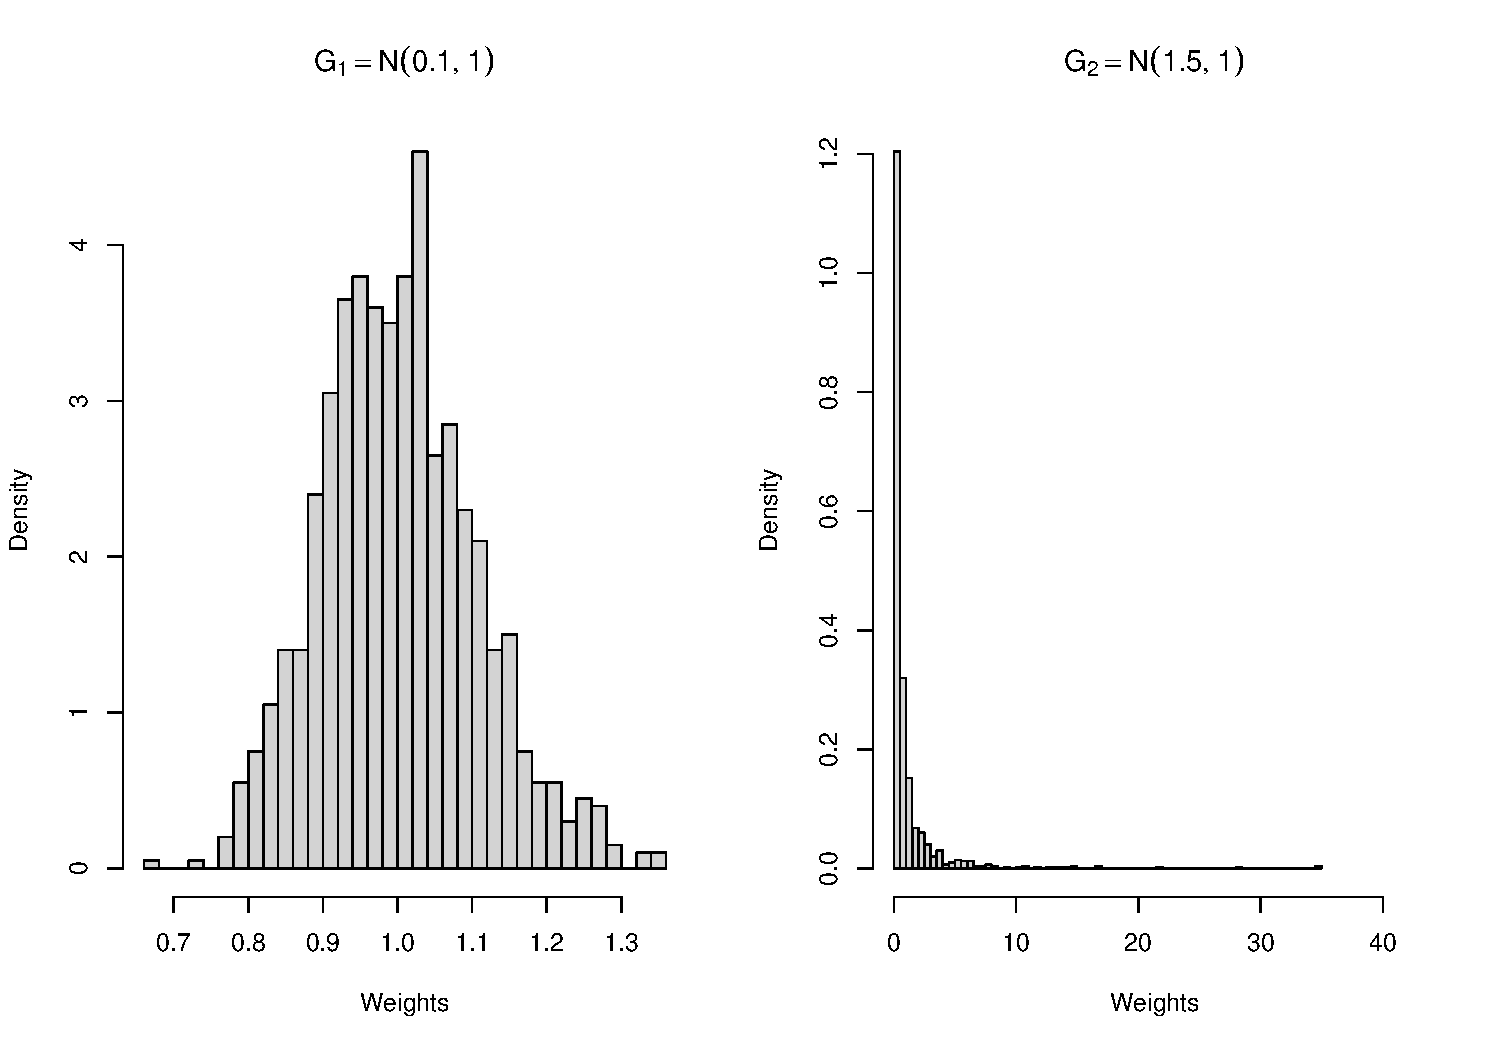
\includegraphics[height=0.9\textheight, width=0.9\textwidth, keepaspectratio]{Figures/Wt Hist - Trunc.pdf}
% \end{frame}

\begin{frame}{Example: Mystery Target}
    \centering
    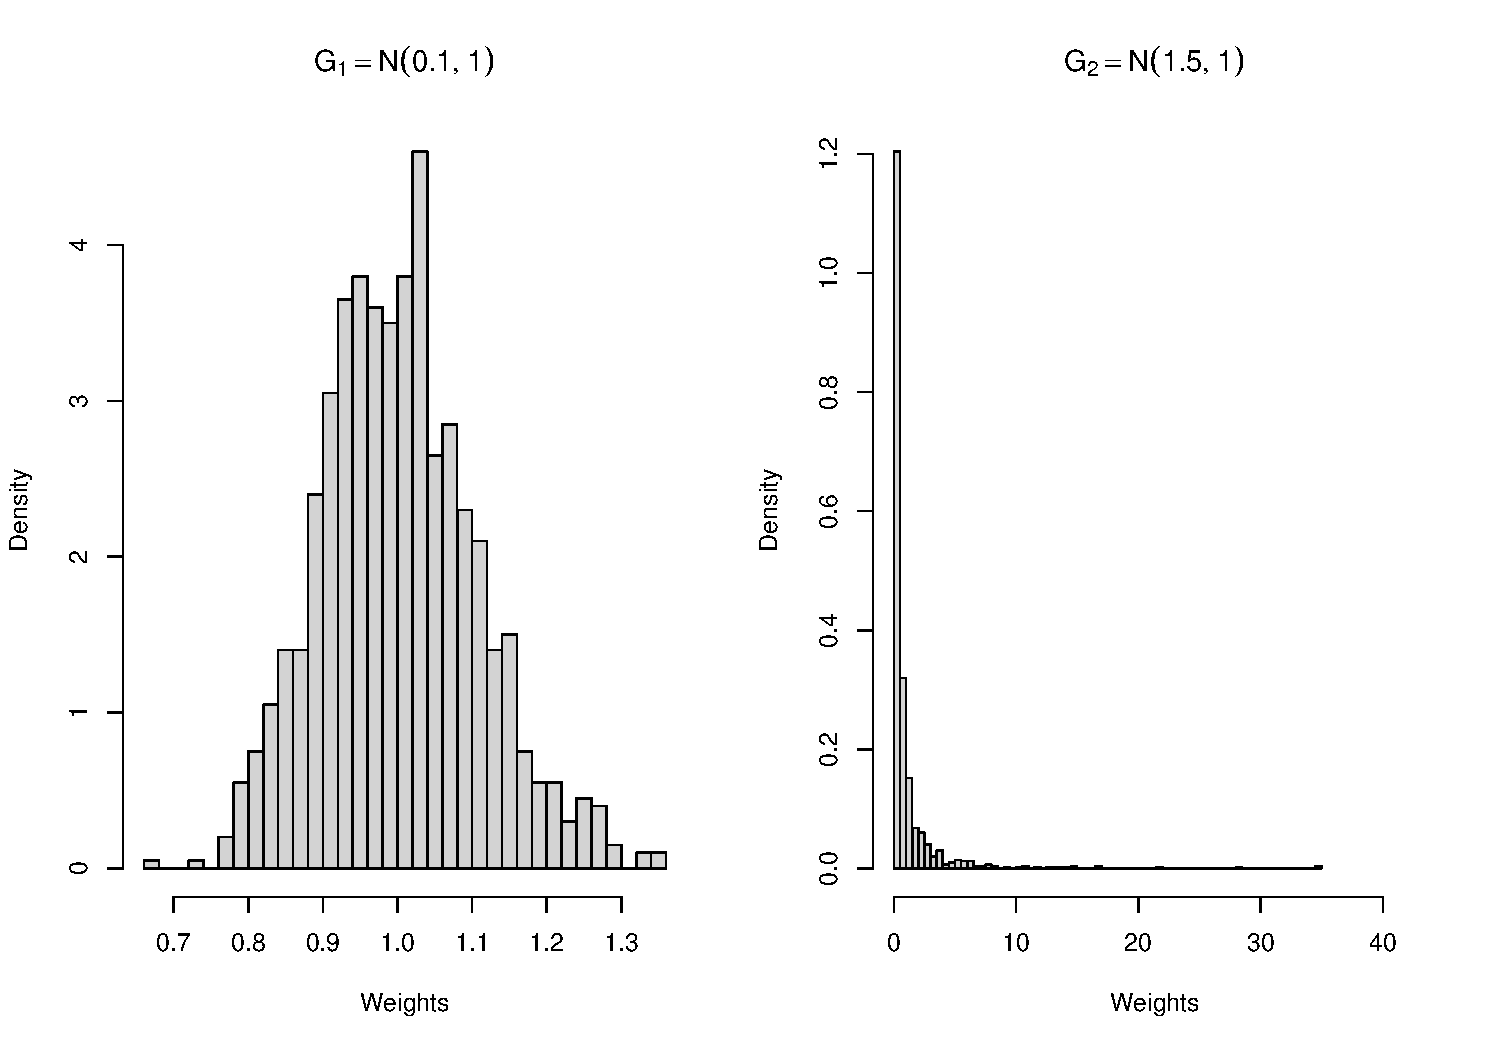
\includegraphics[height=0.7\textheight, width=0.9\textwidth, keepaspectratio]{Figures/Wt Hist - Trunc.pdf} \newline
    \begin{outline}
        $ESS_1 \approx 662$ \hspace{2.5cm} $ESS_2 \approx 54$\\
        $ESS_1^{(\mathrm{trunc})} \approx 662$ \hspace{2.5cm} $ESS_2^{(\mathrm{trunc})} \approx 245$
    \end{outline}
\end{frame}


\begin{frame}{Improving IS}
    \begin{outline}
    \1 Pareto Smoothed Importance Sampling:
        \2 \citep{Veh24} \newline
    \end{outline}

    \setbeamertemplate{enumerate items}[default]
    \begin{enumerate}
    \item Choose a threshold
        \begin{itemize}
            \item Weights above threshold represent tail of their dist.
        \end{itemize}
    \item Approximate tail with Generalized Pareto Dist.
    \begin{itemize}
        \item Fit GPD to weights above threshold
        \item \citep{Zha09}
    \end{itemize}
    \item Replace large weights with quantiles of fitted GPD
    \end{enumerate}
\end{frame}

\begin{frame}{Example: Mystery Target}
    \centering
    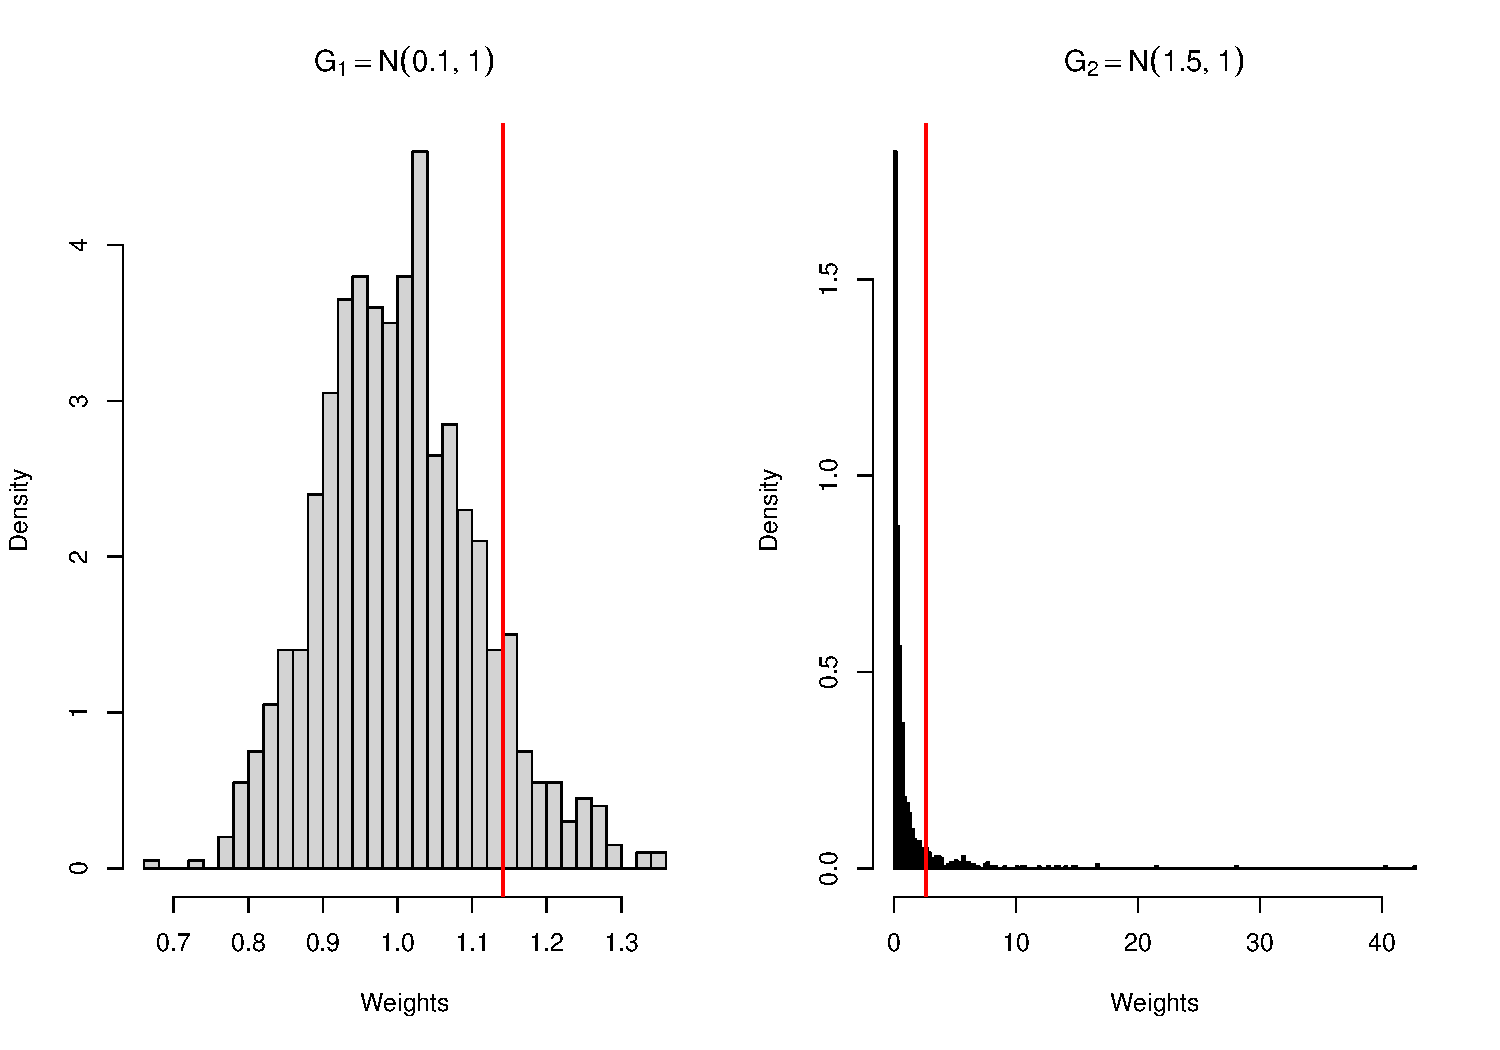
\includegraphics[height=0.9\textheight, width=0.9\textwidth, keepaspectratio]{Figures/Wt Hist - Pareto Thresh.pdf}
\end{frame}

\begin{frame}{Example: Mystery Target}
    \centering
    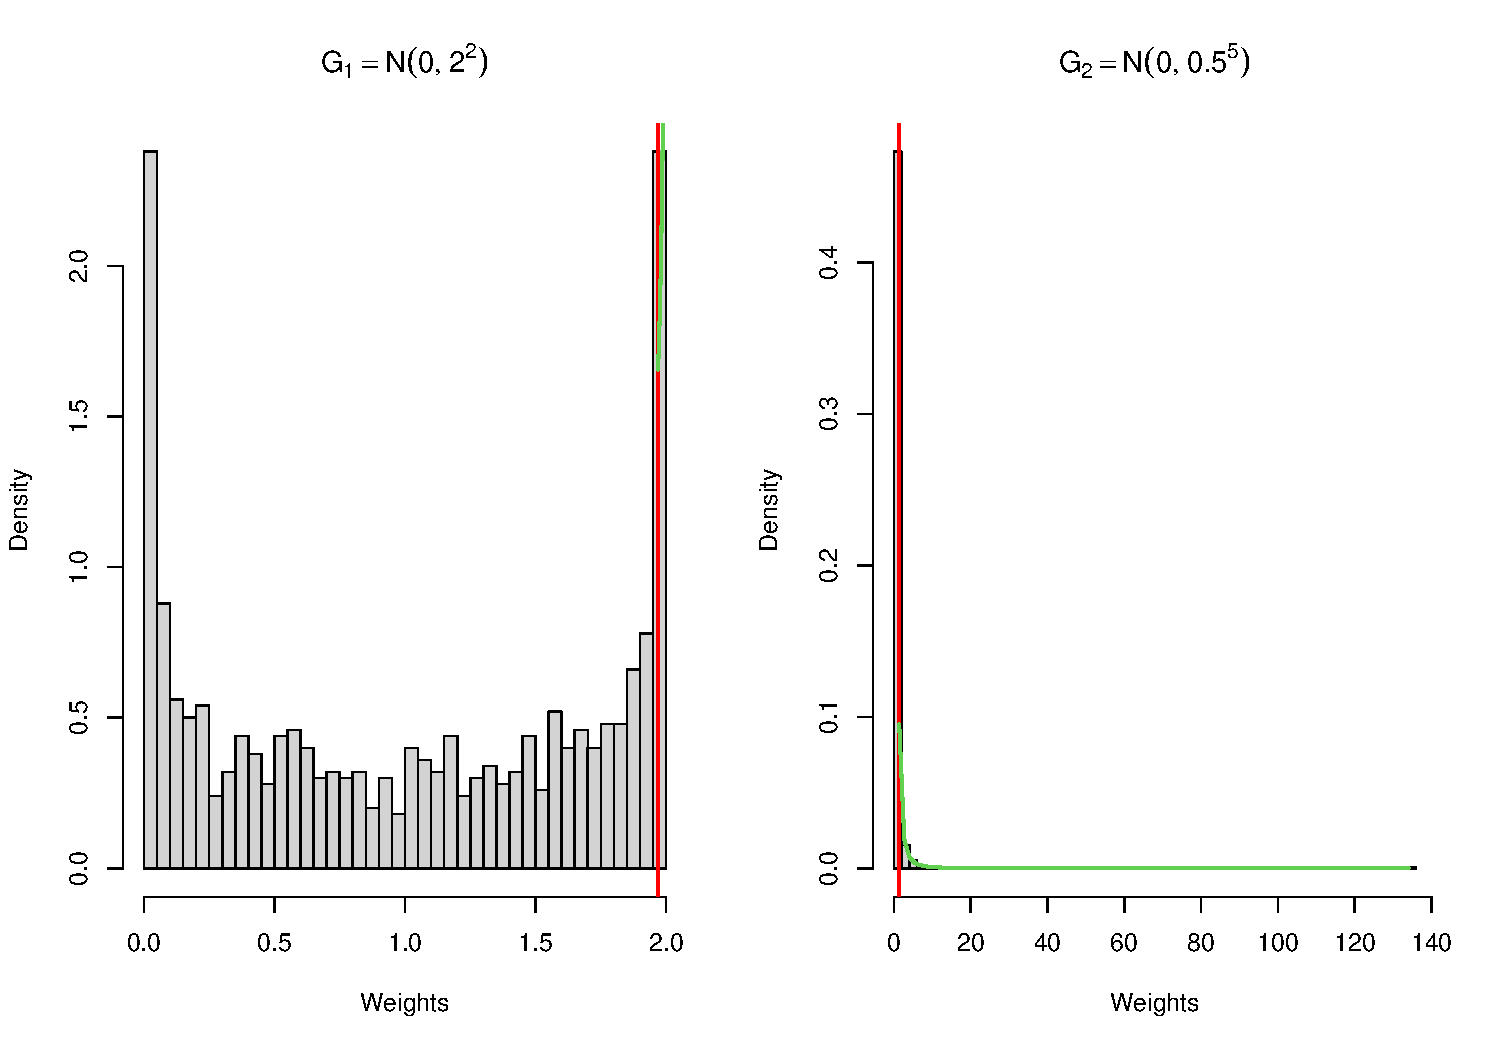
\includegraphics[height=0.7\textheight, width=0.9\textwidth, keepaspectratio]{Figures/Wt Hist - Pareto Dens.pdf} \newline
    \begin{outline}
        $\hat{k}_1 \approx -1.81$ \hspace{2cm} $\hat{k}_2 \approx 0.72$
    \end{outline}
\end{frame}

\begin{frame}{Example: Mystery Target}
    \centering
    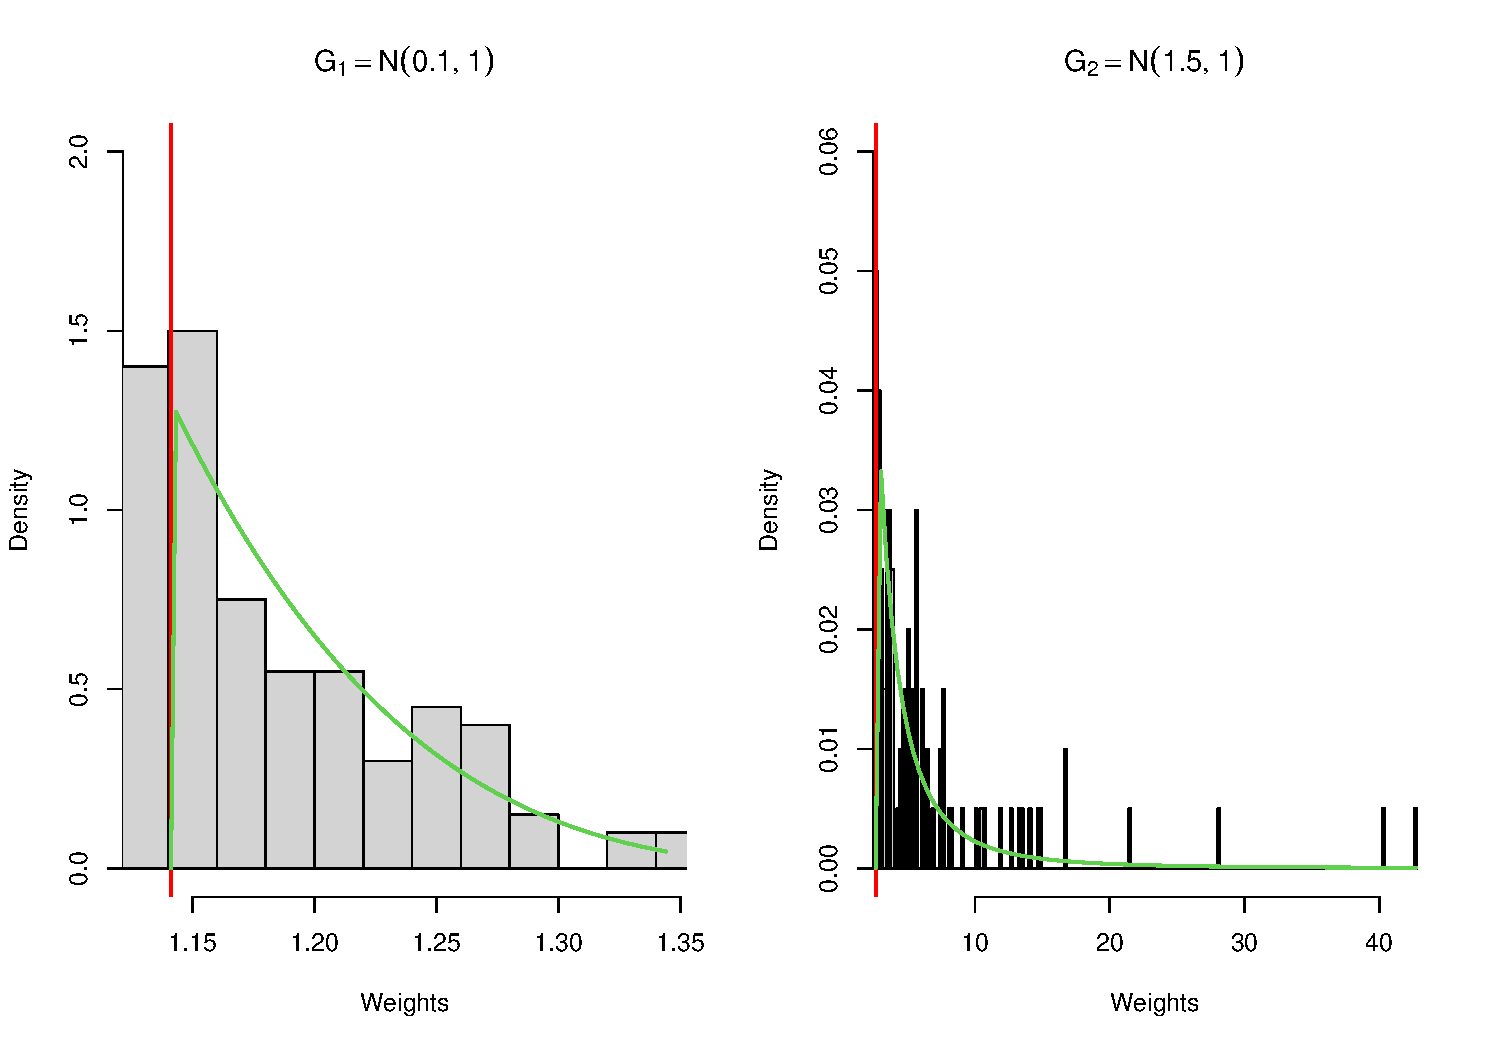
\includegraphics[height=0.9\textheight, width=0.9\textwidth, keepaspectratio]{Figures/Wt Hist - Pareto Dens Zoom.pdf}
\end{frame}

\begin{frame}{Example: Mystery Target}
    \centering
    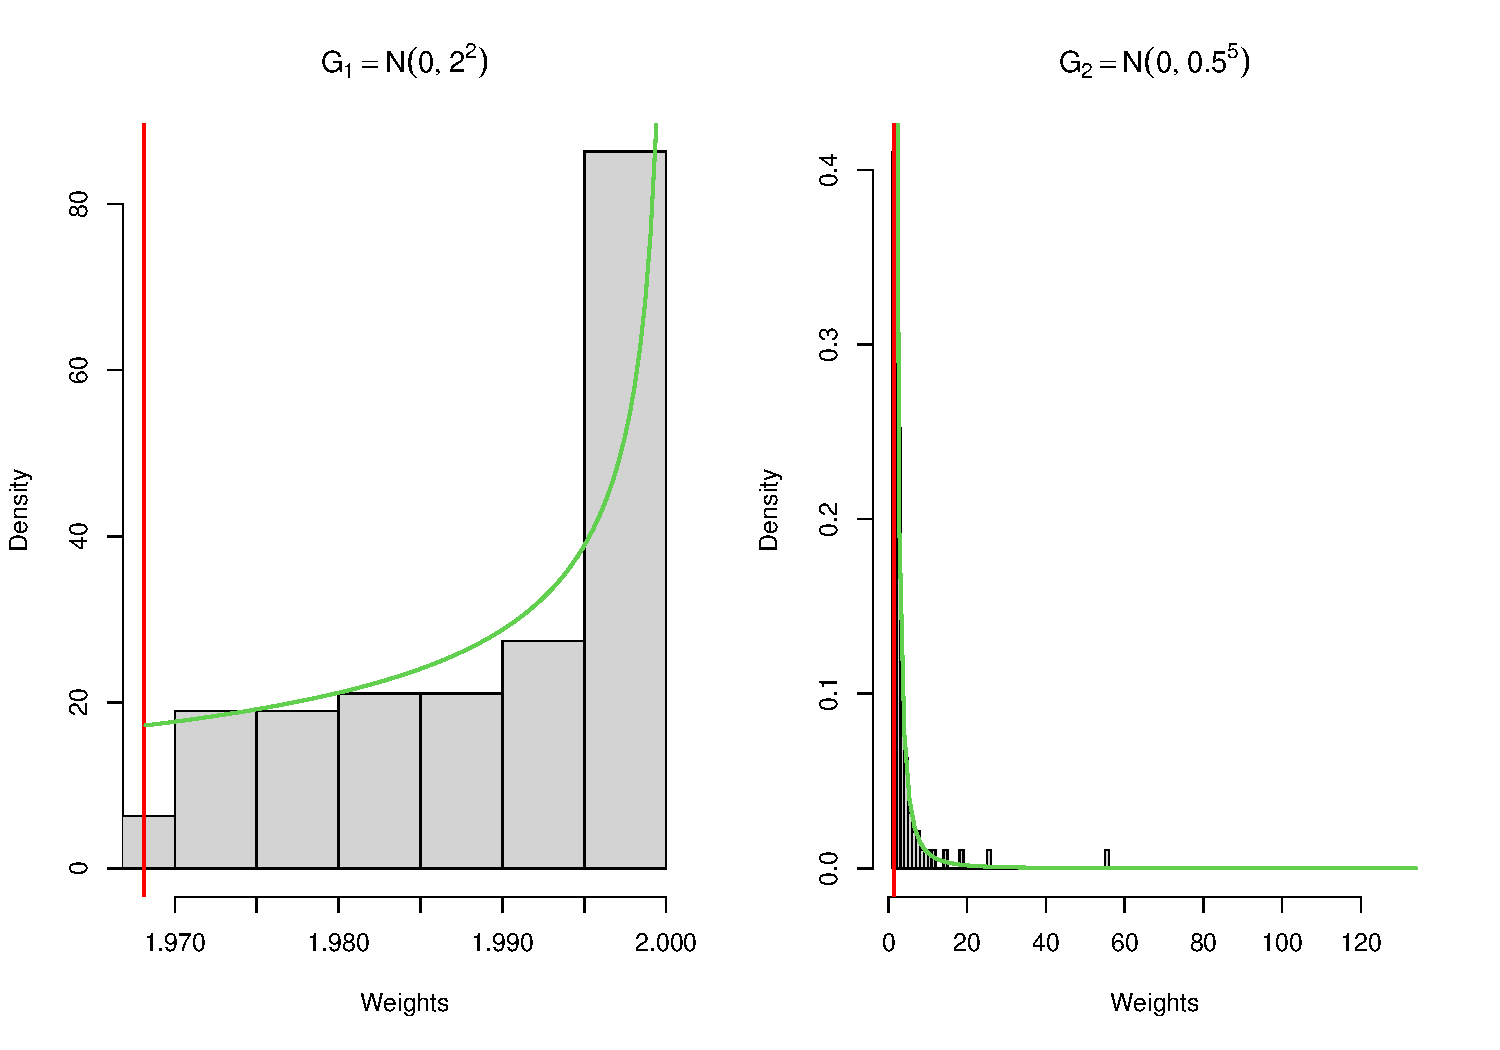
\includegraphics[height=0.9\textheight, width=0.9\textwidth, keepaspectratio]{Figures/Wt Hist - Pareto Smooth Zoom.pdf}
\end{frame}

\begin{frame}{Example: Mystery Target}
    \centering
    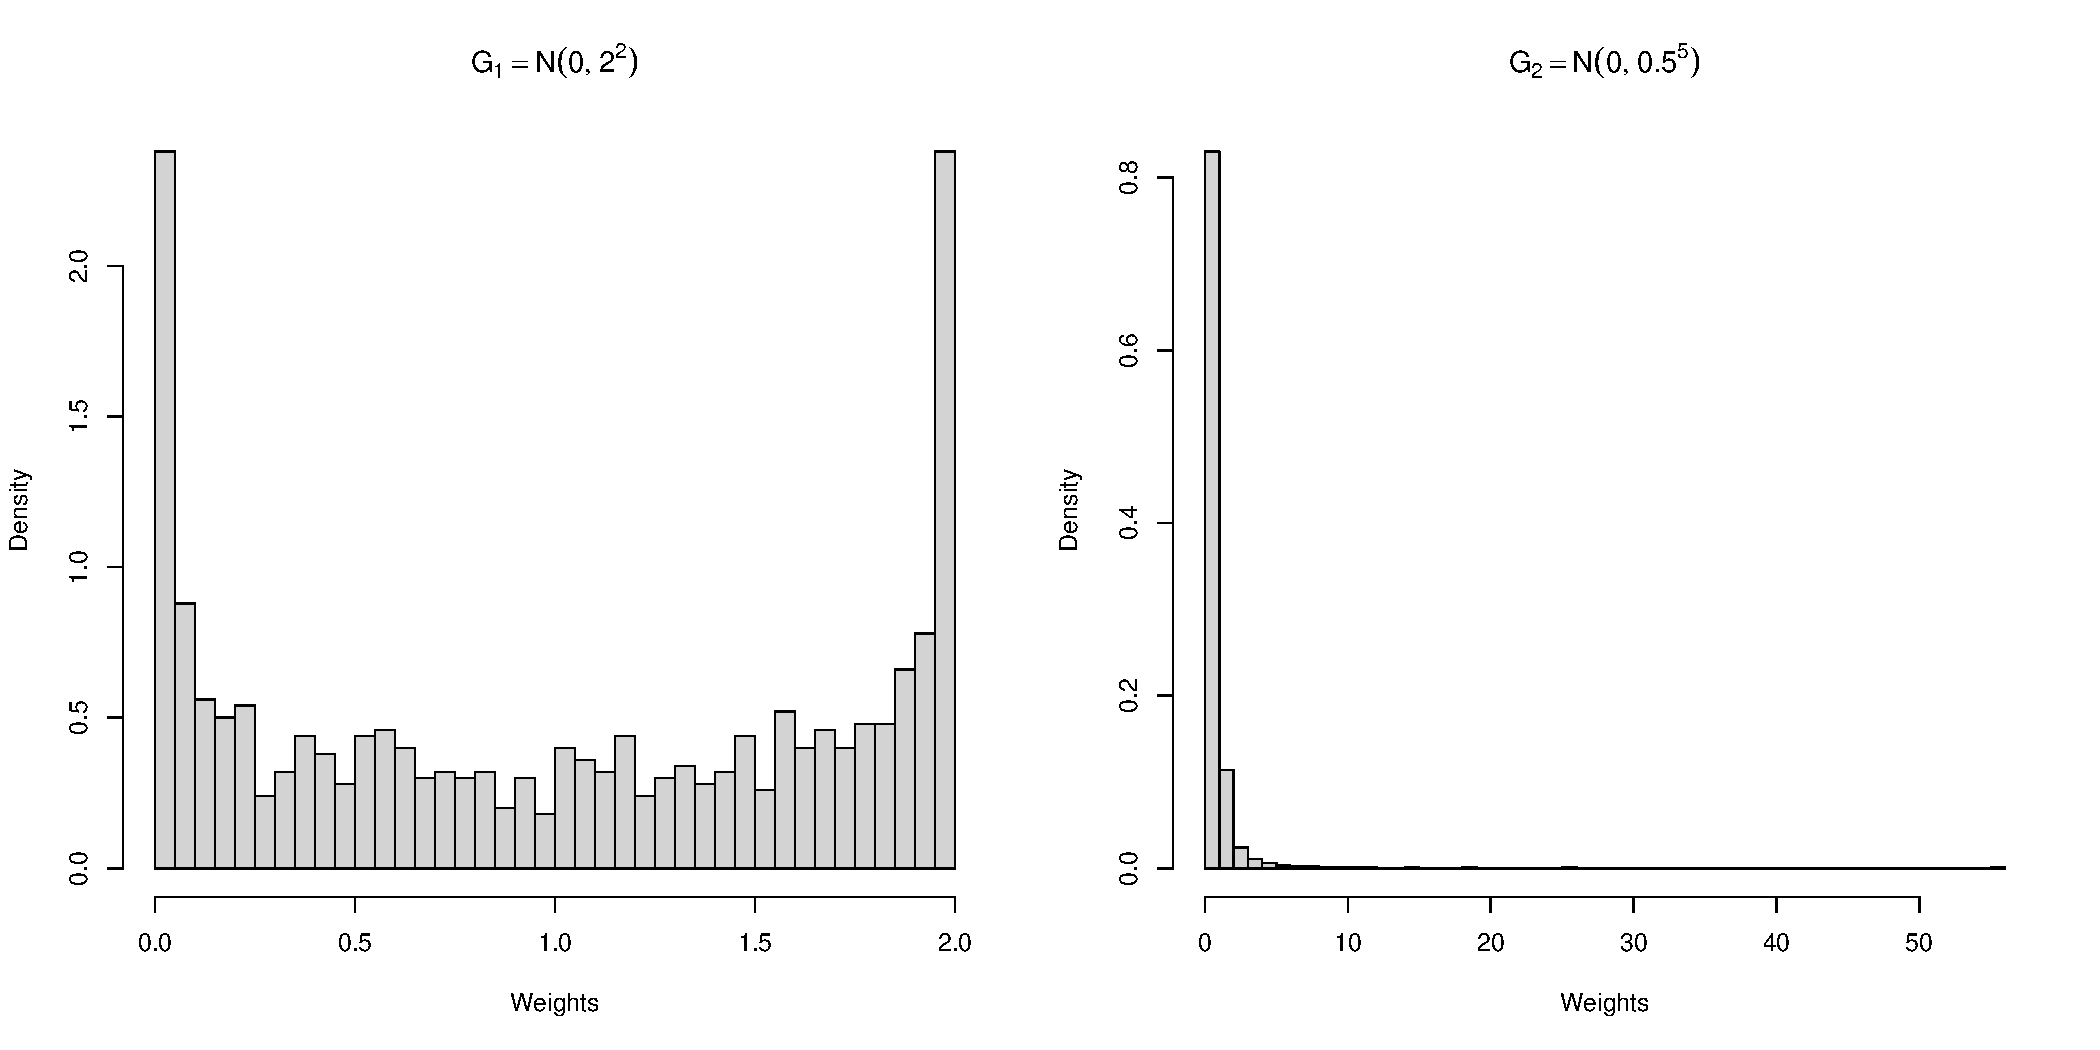
\includegraphics[height=0.5\textheight, width=0.9\textwidth]{Figures/Wt Hist - Pareto Smooth.pdf}\newline
    \begin{outline}
        $ESS_1 \approx 662$ \hspace{2.5cm} $ESS_2 \approx 54$\\
        $ESS_1^{(\mathrm{trunc})} \approx 662$ \hspace{2.5cm} $ESS_2^{(\mathrm{trunc})} \approx 245$\\
        $ESS_1^{(\mathrm{PS})} \approx 662$ \hspace{2.5cm} $ESS_2^{(\mathrm{PS})} \approx 160$
    \end{outline}
\end{frame}


\begin{frame}{Adaptive IS}
    \begin{outline}
        \1 Alternative approach: directly optimize ESS \newline

        \1 Adaptive Importance Sampling: 
            \2 \citep{Aky21} \newline
    \end{outline}

    \begin{enumerate}
        \setbeamertemplate{enumerate items}[default]
        \item Choose a (parametric) family of proposals
        \item Iteratively update the proposal to maximize ESS
    \end{enumerate}
\end{frame}

\begin{frame}{Stochastic Approximation}
    \begin{outline}
        \1 Actually, minimize a population-level analog: 
            \2 $\rho = \bE_G w^2(X) \approx \frac{N}{ESS}$ \newline

        \1 If we had $\rho$, we would do gradient descent
            \2 $\theta_{k+1} = \theta_k - \alpha_k \nabla \rho(\theta_k)$ \newline

        \1 Instead, do gradient descent on $\hat{\rho}$
            \2 $\hat{\theta}_{k+1} = \hat{\theta}_k - \alpha_k \nabla \hat{\rho}(\hat{\theta}_k)$ 
        \1 Stochastic approximation
    \end{outline}
\end{frame}


\begin{frame}{Stochastic Approximation}
    \begin{outline}
        \1 Originally developed for root finding with noise
            \2 \citep{Rob51} \newline

        \1 Quickly adapted for optimization
            \2 Use noisy evaluations for finite difference
            \2 \citep{Kie52} 
    \end{outline}
\end{frame}

\begin{frame}{Stochastic Approximation}
    \begin{outline}
        \1 Very well developed theory
        \1 Step size $\rightarrow$ 0
            \2 Called the ``learning rate'' \newline

        \1 Stochastic gradient descent
            \2 Popular in machine learning
            \2 Resample a (very) large dataset

    \end{outline}
\end{frame}

\begin{frame}{Example: Mystery Target}
    \centering
    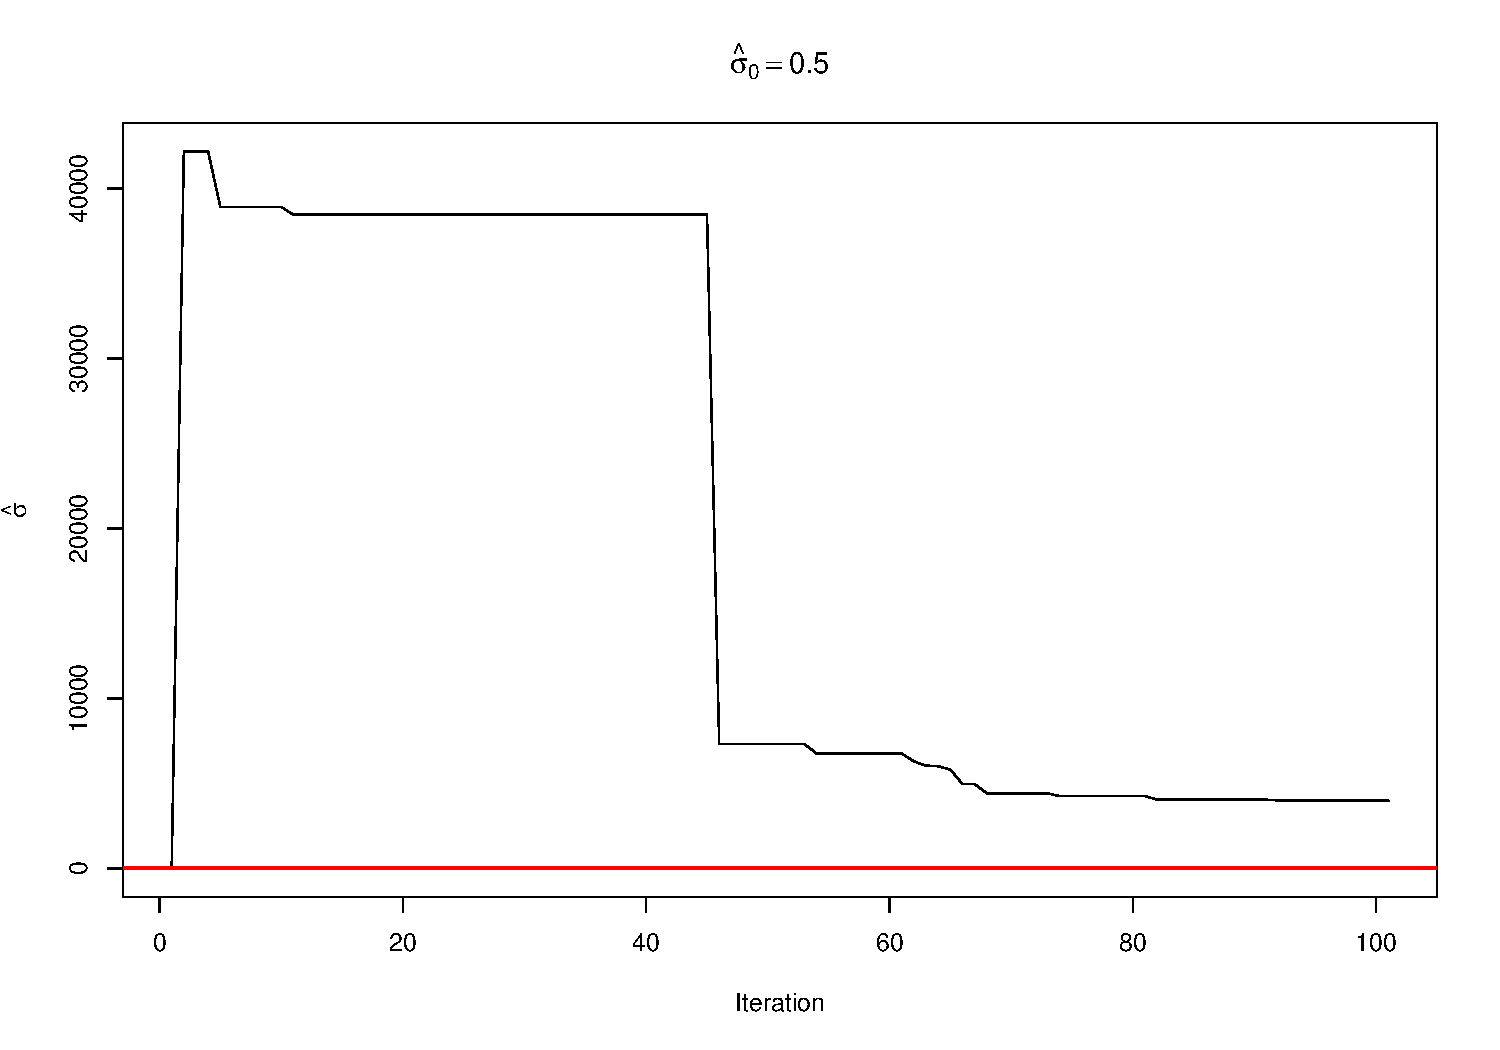
\includegraphics[height=0.9\textheight, width=0.9\textwidth, keepaspectratio]{Figures/ESS Traj - 0,5.pdf}
\end{frame}

\begin{frame}{Example: Mystery Target}
    \centering
    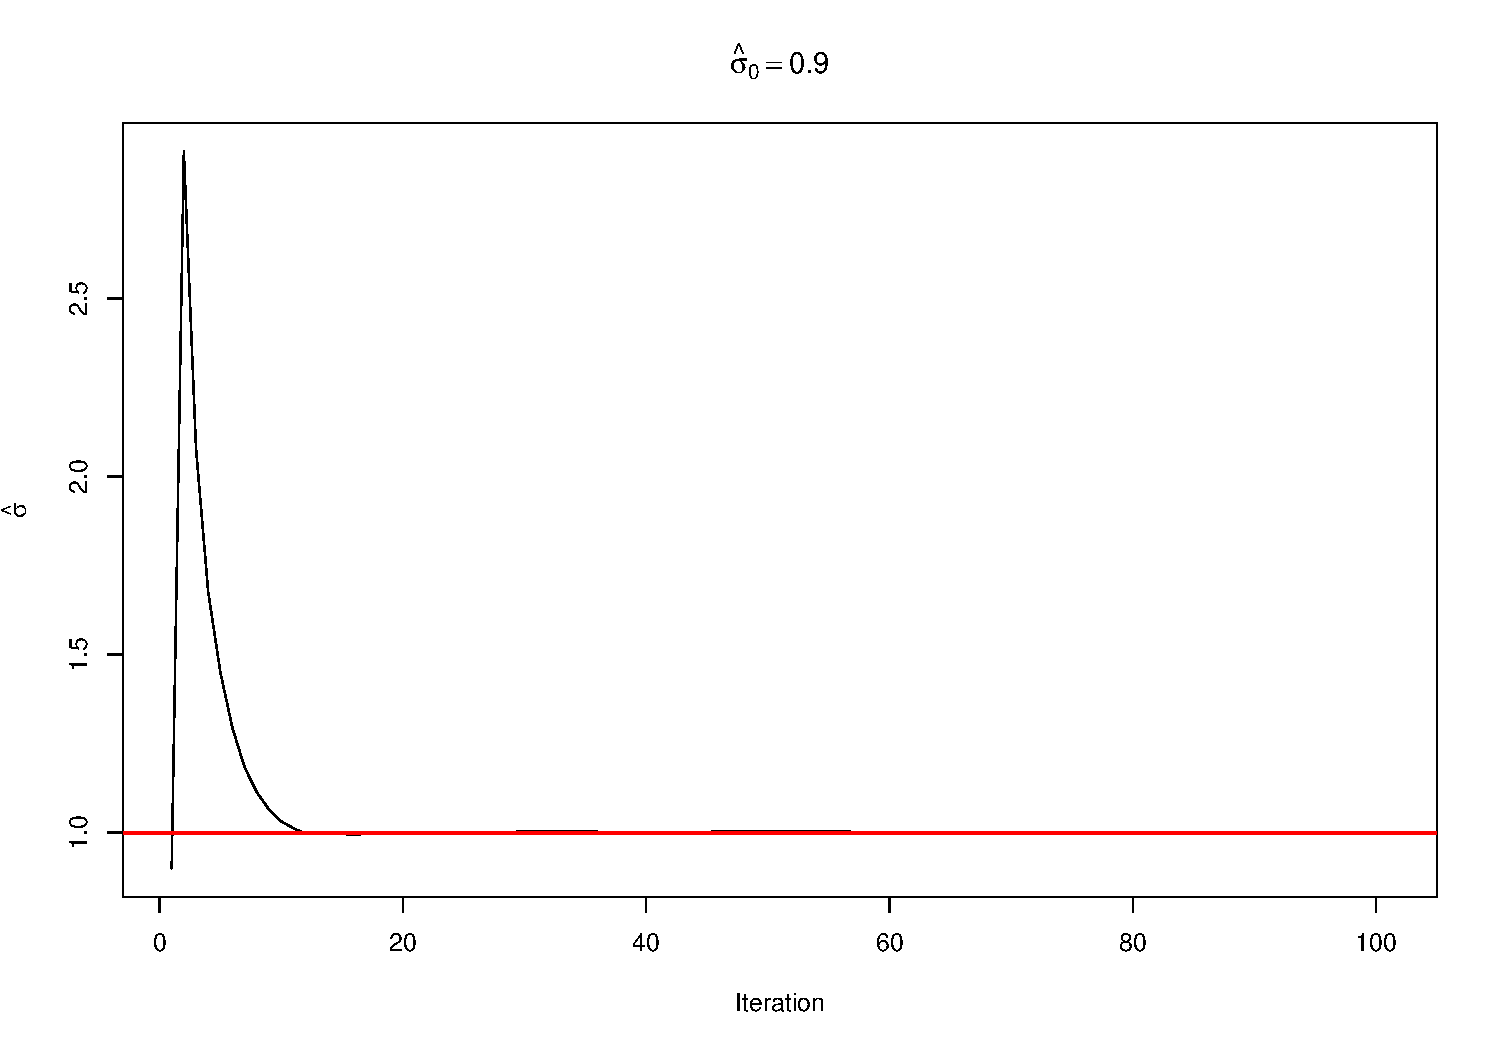
\includegraphics[height=0.9\textheight, width=0.9\textwidth, keepaspectratio]{Figures/ESS Traj - 0,9.pdf}
\end{frame}

\begin{frame}{Example: Mystery Target}
    \centering
    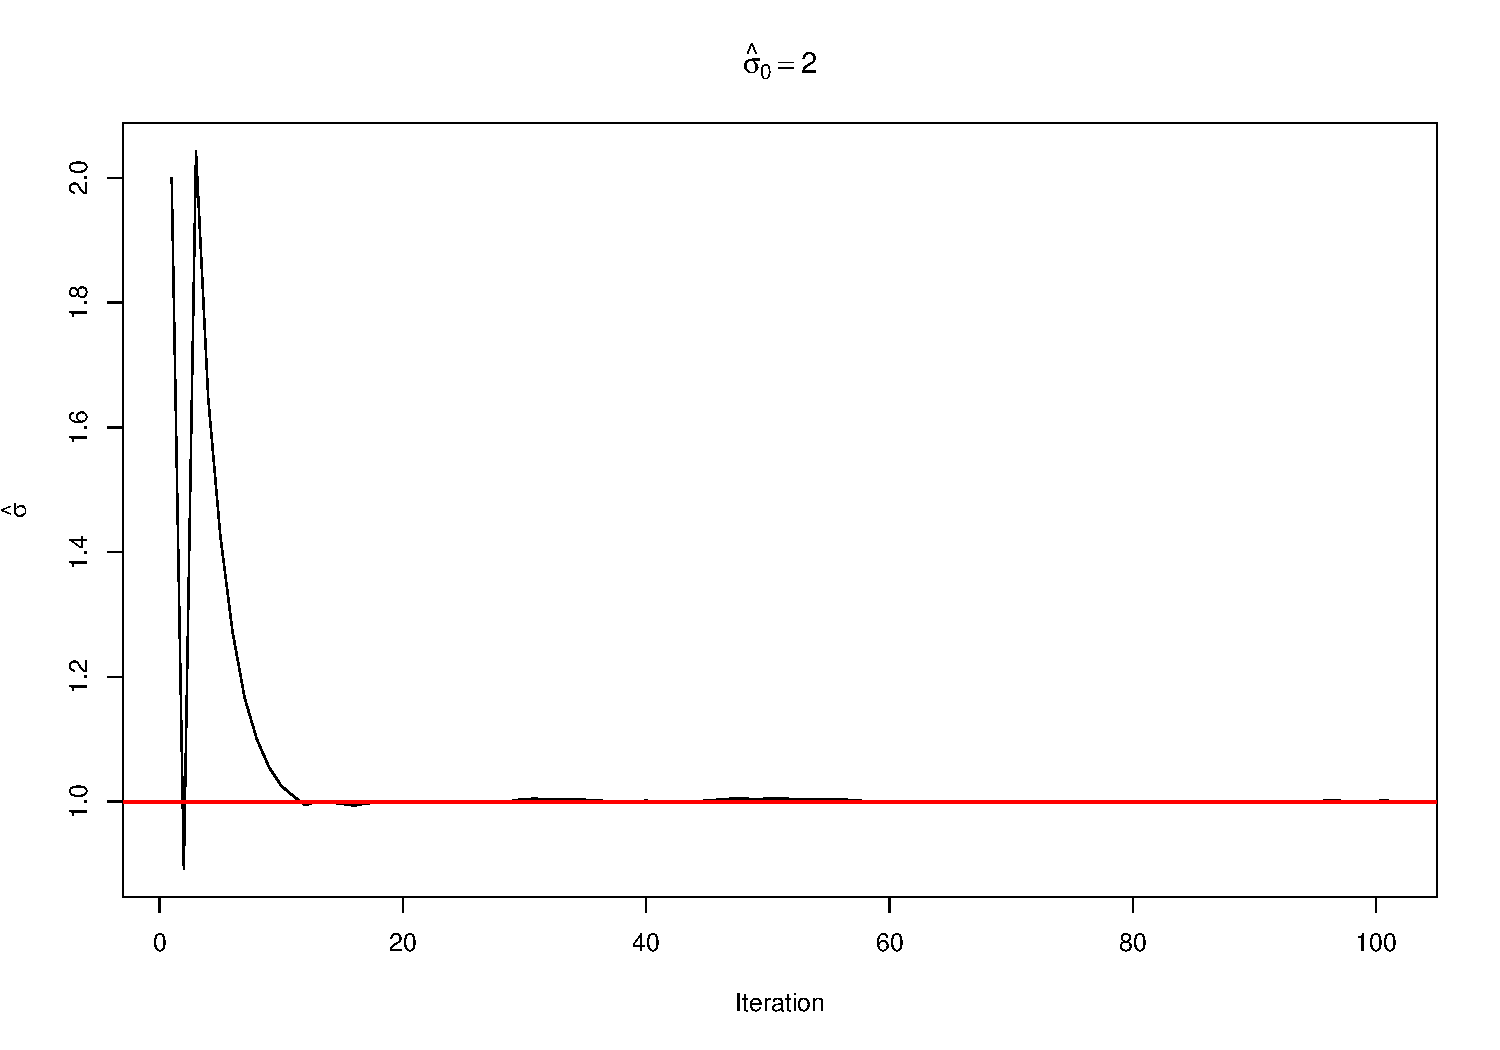
\includegraphics[height=0.9\textheight, width=0.9\textwidth, keepaspectratio]{Figures/ESS Traj - 2.pdf}
\end{frame}

\begin{frame}{Example: Mystery Target}
    \centering
    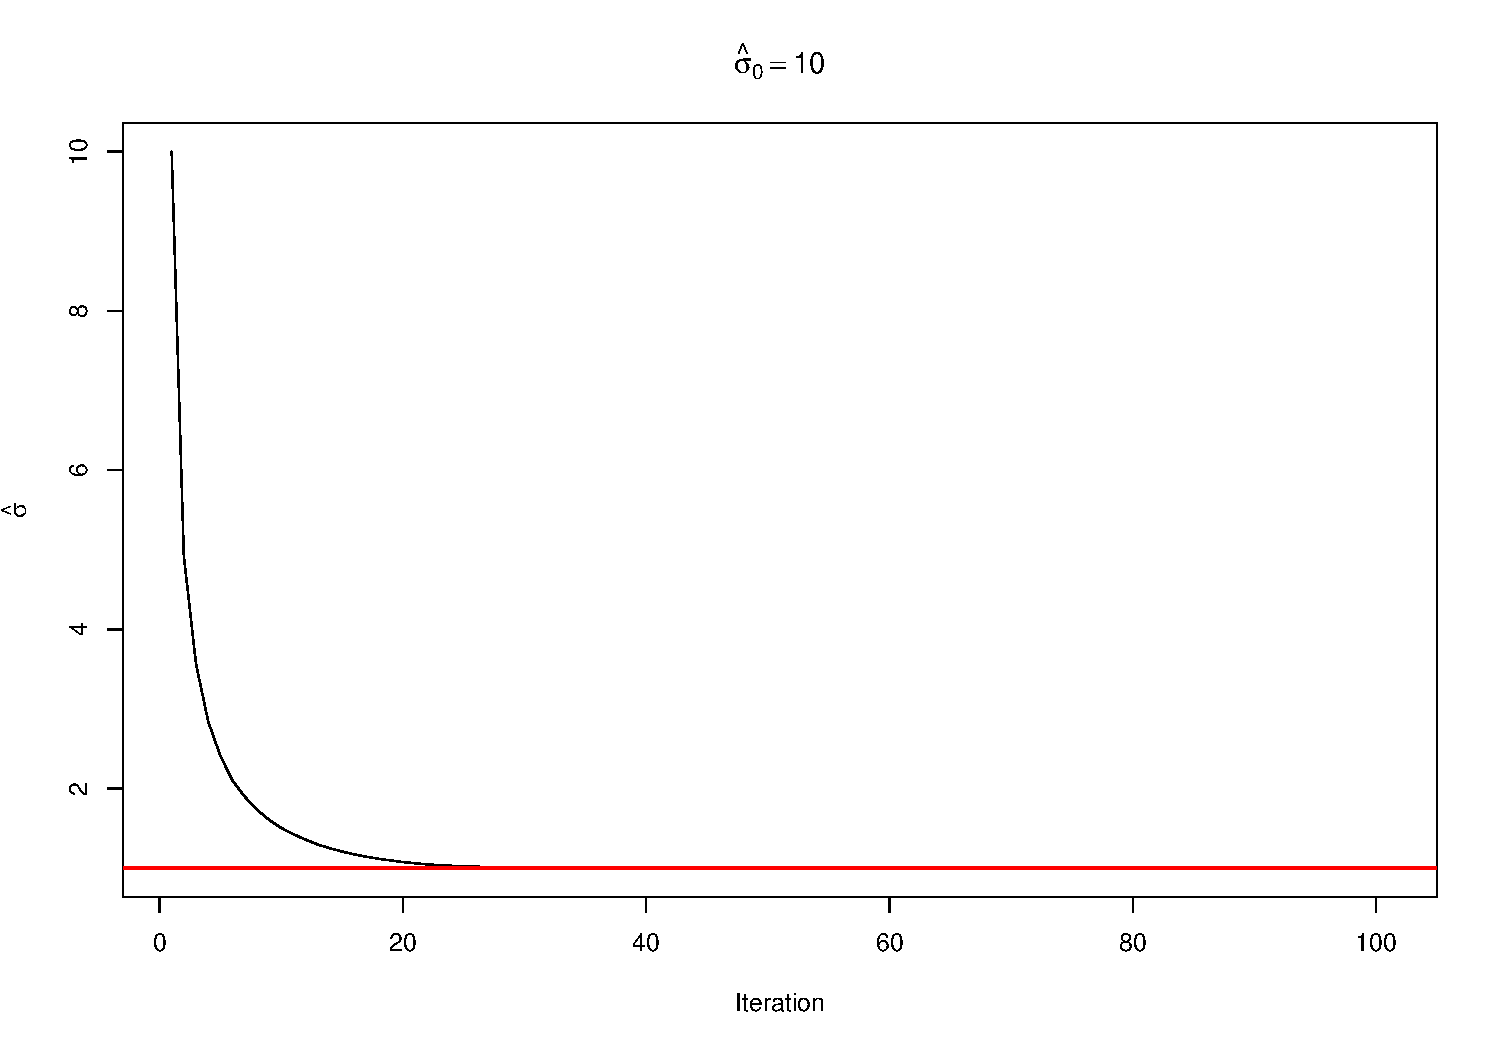
\includegraphics[height=0.9\textheight, width=0.9\textwidth, keepaspectratio]{Figures/ESS Traj - 10.pdf}
\end{frame}


%! This resembles the previous slide
% \begin{frame}{Example: Mystery Target}
%     \centering
%     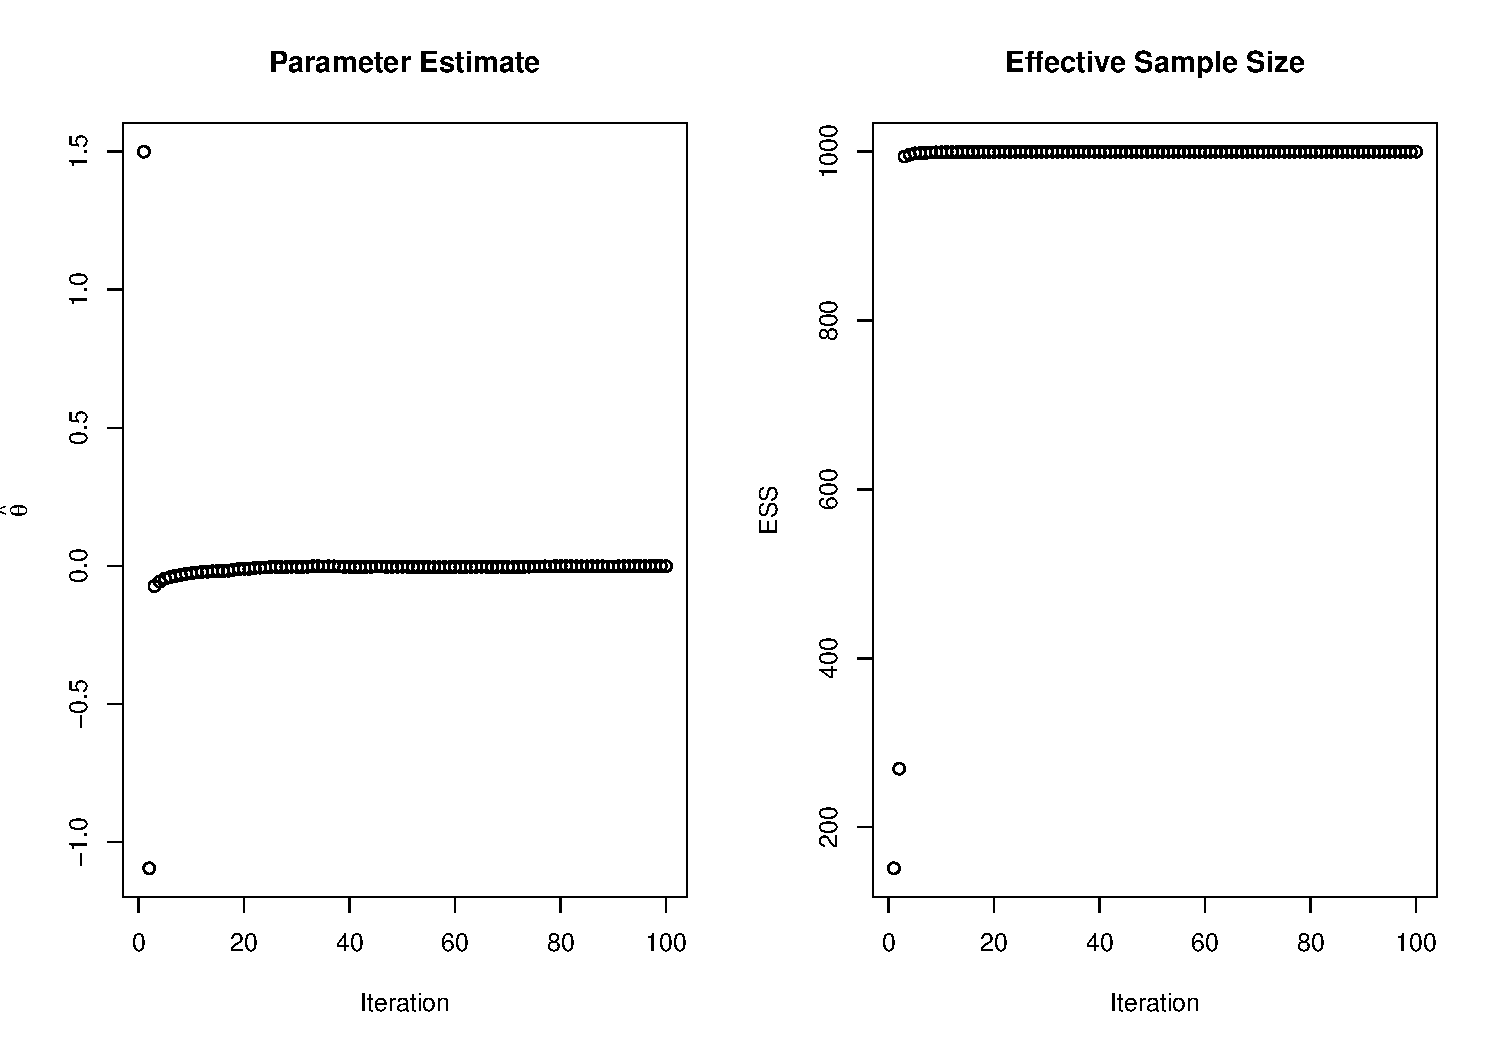
\includegraphics[height=0.7\textheight, width=0.9\textwidth, keepaspectratio]{Figures/ESS traj.pdf} \newline
%     \begin{outline}
%         $\hat{\theta}_\mathrm{end}^{(ESS)} \approx -8 \times 10^{-4}$ \hspace{1cm} $ESS_\mathrm{end} \approx 1000 - (7 \times 10^{-4})$
%     \end{outline}
% \end{frame}


\begin{frame}{Our Method}
    \begin{outline}
        \1 Recall: Be careful using IS means to diagnose IS \newline
        
        \1 \citeauthor{Veh22} give an alternative
            \2 Shape parameter of fitted tail distribution, $\hat{k}$
    \end{outline}
\end{frame}


%! Consider adding this back in. I haven't yet found a way to present the numerics that I feel confident about
% \begin{frame}{Our Method}
%     \begin{outline}
%         \1 Consider repeated sampling with $\sigma = 0.5$ (hard)
%         \1 For each sample, estimate $\rho$ and $k$ \newline

%         \1 Coefficient of Variation:
%             \2 $\hat{\rho}$: $5.06$
%             \2 $\hat{k}$: $0.22$
%     \end{outline}
    
% %     \centering
% %   \begin{tabular}{|c|c c|}
% %     \hline
% %     & $\hat{\rho}$ & $\hat{k}$ \\
% %     \hline
% %     Mean & 29.6 & 0.65 \\ 
% %     Standard Error & 15.0 & 0.01 \\ 
% %     Coefficient of Variation & {5.1} & {0.22}\\
% %     \hline
% %   \end{tabular}
% \end{frame}

% \begin{frame}{Our Method}
%     \centering
%   \begin{tabular}{|c|c c|}
%     \hline
%     & $\hat{\rho}$ & $\hat{k}$ \\
%     \hline
%     Mean & 29.6 & 0.65 \\ 
%     Standard Error & 15.0 & 0.01 \\ 
%     \textbf{Coefficient of Variation} & \textbf{5.1} & \textbf{0.22}\\
%     \hline
%   \end{tabular}
% \end{frame}

\begin{frame}{Our Method}
    \begin{outline}
        \1 Use diagnostic as objective function \newline

        \1 Apply stochastic approximation to minimize $\hat{k}$
            \2 More precisely, its population analog: $k(\theta)$ \newline

        \1 Use finite difference approximation to $\hat{k}'(\theta)$
            \2 This is subtle
    \end{outline}
\end{frame}

\begin{frame}{Example: Mystery Target}
    \centering
    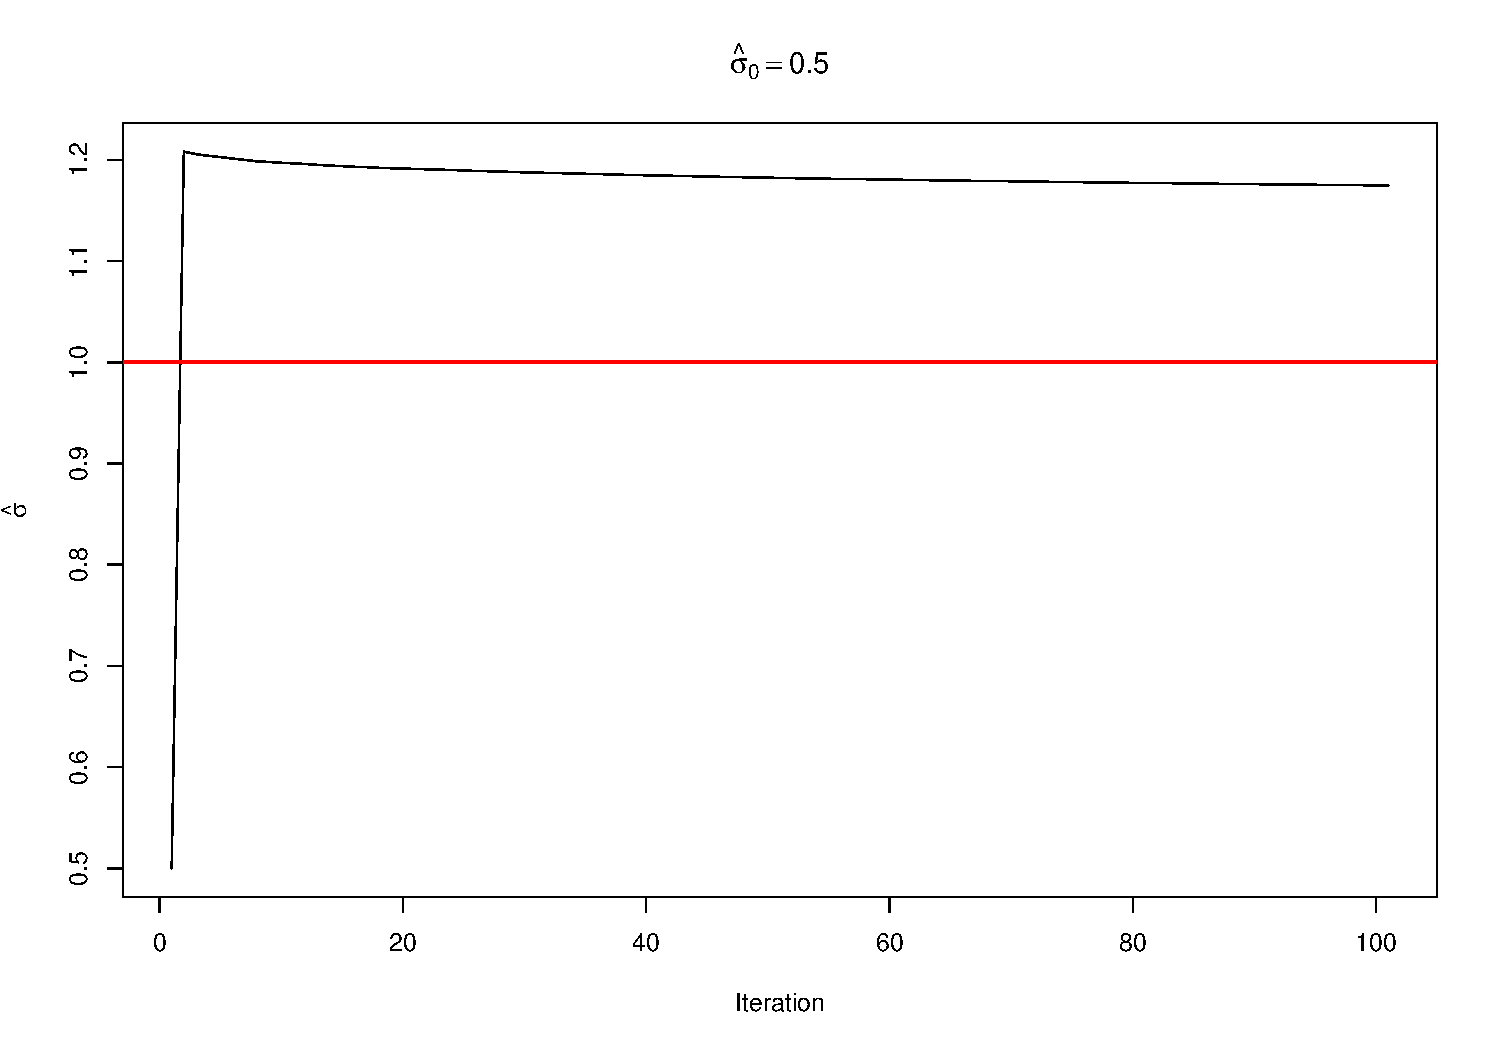
\includegraphics[height=0.9\textheight, width=0.9\textwidth, keepaspectratio]{Figures/k_hat Traj - 0,5.pdf}
\end{frame}

\begin{frame}{Example: Mystery Target}
    \centering
    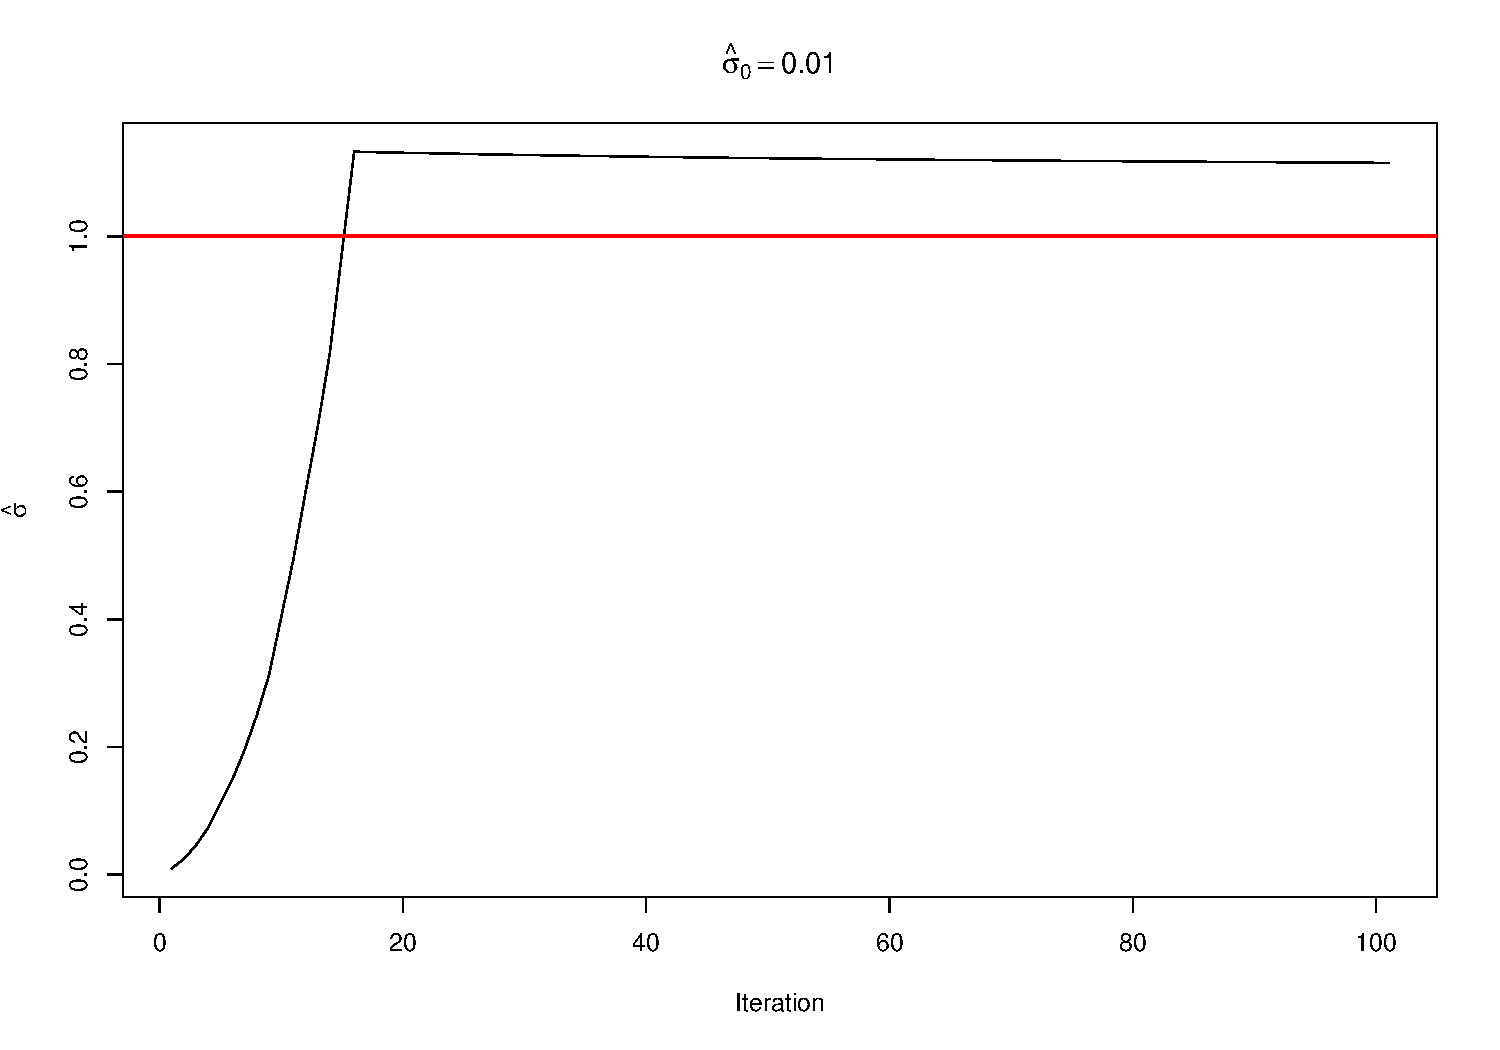
\includegraphics[height=0.9\textheight, width=0.9\textwidth, keepaspectratio]{Figures/k_hat Traj - 0,01.pdf}
\end{frame}

\begin{frame}{Example: Mystery Target}
    \centering
    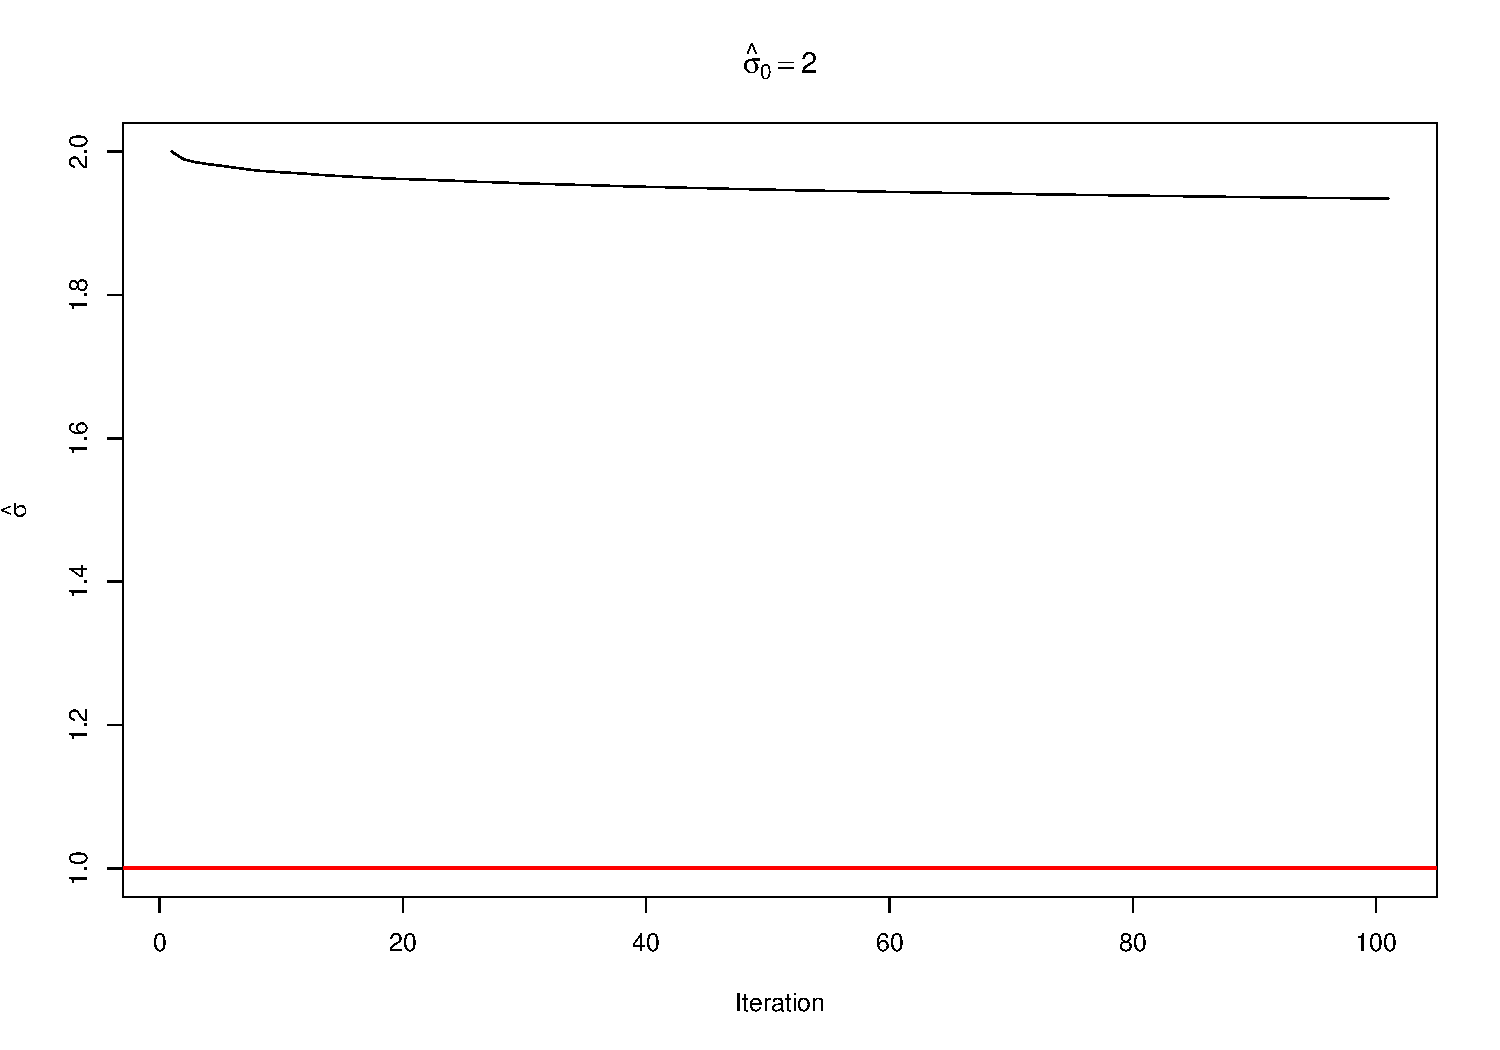
\includegraphics[height=0.9\textheight, width=0.9\textwidth, keepaspectratio]{Figures/k_hat Traj - 2.pdf}
\end{frame}

\begin{frame}{Our Method - Future Directions}
    \begin{outline}
        \1 Refining the finite difference approximation
            \2 Generalize ESS version outside exponential families \newline

        \1 Analytical tail indices
        \1 Convergence theory for stochastic approximation \newline

        \1 Applications
            \2 Latent variable models (e.g. GLMMs)
            \2 Bayesian inference in high-dimensions
    \end{outline}
\end{frame}


\begin{frame}{Recap}
    \begin{outline}
        \1 Importance sampling and extensions
            \2 Truncation
            \2 Pareto Smoothing \newline
        
        \1 Diagnostics for importance sampling
            \2 Effective sample size
            \2 Pareto tail index \newline

        \1 Adaptive importance sampling
            \2 Stochastic approximation
    \end{outline}
\end{frame}



\begin{frame}{Topics}
    \begin{outline}
        \1 Adaptive Pareto Smoothed Importance Sampling \newline
        \1 \textbf{Multilevel Causal Mediation Analysis} \newline
        \1 Modelling Tuberculosis in Foreign-Born Canadians
    \end{outline}
\end{frame}

\begin{frame}{Outline}
    \begin{itemize}
        \setlength{\itemsep}{0.75em}
        \item[1)] The Problem
        \item[2)] Mediation Analysis
        \item[3)] Causal Inference
        \item[4)] Mixed-Effects Models
        \item[5)] Mixed-Effects Models in Causal Mediation Analysis
    \end{itemize}
\end{frame}

\begin{frame}{Example}
    \begin{itemize}
        \item Goal: Understand adherence to restrictive measures
        \begin{itemize}
            \item E.g. Lockdowns
            \item Both past and future \newline
        \end{itemize}
        \item Influence of news source
        \begin{itemize}
            \item How trustworthy? \newline
        \end{itemize}
        \item Disentangle influence on future from influence on past
    \end{itemize}
    
\end{frame}


\begin{frame}{Example}
        \begin{figure}[H]
            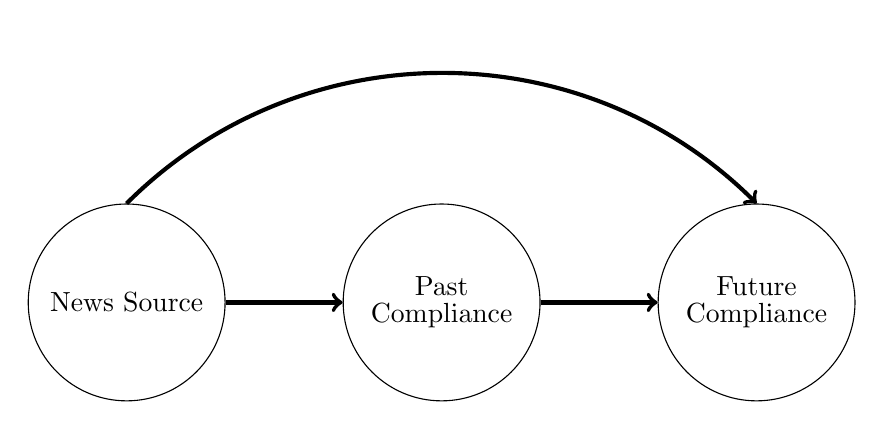
\begin{tikzpicture}
                % Circles with labels
                \node at (0,0) [circle, draw, minimum size=2.5cm] (news) {News Source};
                \node at (4,0) [circle, draw, minimum size=2.5cm] (past) {\shortstack{Past\\Compliance}};
                \node at (8,0) [circle, draw, minimum size=2.5cm] (future) {\shortstack{Future\\Compliance}};
                
                % Arrows
                \draw[->, line width=1.5pt] (news.east) -- (past.west);
                \draw[->, line width=1.5pt] (past.east) -- (future.west);
                \draw[->, line width=1.5pt, bend left] (news.north) to [out=45,in=135] (future.north); 
                
                \end{tikzpicture}
    \end{figure}
\end{frame}

\begin{frame}{Example}
    Terminology
    \begin{columns}
        \column{0.6\textwidth}
        \begin{itemize}
            \item Top path: {Direct effect}
            \item Center path: {Indirect effect}
            \item Combined: {Total effect}
        \end{itemize}
        \column{0.4\textwidth}
        \begin{itemize}
            \item Exposure: $X$
            \item Outcome: $Y$
            \item Mediator: $M$
        \end{itemize}
    \end{columns}
    
\end{frame}




\begin{frame}{Mediation Analysis}
    \begin{figure}[H]
        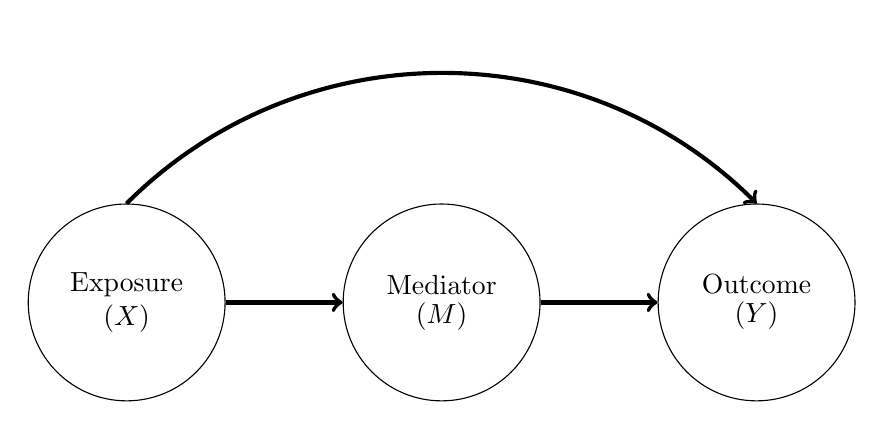
\begin{tikzpicture}
            % Circles with labels
            \node at (0,0) [circle, draw, minimum size=2.5cm] (X) {\shortstack{Exposure\\($X$)}};
            \node at (4,0) [circle, draw, minimum size=2.5cm] (M) {\shortstack{Mediator\\($M$)}};
            \node at (8,0) [circle, draw, minimum size=2.5cm] (Y) {\shortstack{Outcome\\($Y$)}};
            
            % Arrows
            \draw[->, line width=1.5pt] (X.east) -- (M.west);
            \draw[->, line width=1.5pt] (M.east) -- (Y.west);
            \draw[->, line width=1.5pt, bend left] (X.north) to [out=45,in=135] (Y.north); 
            
            \end{tikzpicture}
    \end{figure}
\end{frame}

\begin{frame}{Mediation Analysis}
    Separate \textbf{Total Effect} of $X$ on $Y$ into
    \begin{itemize}
        \item \textbf{Direct Effect}
        \item \textbf{Indirect Effect}\newline
    \end{itemize}

    Traditionally, use regression
\end{frame}

\begin{frame}{Mediation Analysis}
    Continuous outcome and mediator:
    \begin{itemize}
        \item $Y = \alpha_0 + \alpha_1 M + \alpha_2 X + \varepsilon_Y$
        \item $M = \beta_0 + \beta_1 X + \varepsilon_M$ \newline
    \end{itemize}

    
    \textbf{Direct Effect}: $\alpha_2$
    \begin{itemize}
        \item ``$X$ in $Y$''
    \end{itemize}
    \textbf{Indirect Effect}: $\alpha_1 \cdot \beta_1$
    \begin{itemize}
        \item ``$M$ in $Y$'' $\cdot$ ``$X$ in $M$''
    \end{itemize}
    \textbf{Total Effect}: $\alpha_2 + \alpha_1 \cdot \beta_1$

\end{frame}

\begin{frame}{Mediation Analysis}
    Popular approach
    \begin{itemize}
        \item A bit outdated\ldots \newline
    \end{itemize}

    More popular: Causal mediation analysis
    
\end{frame}

\begin{frame}{Causal Inference}
    Assume that $X$ \textit{causes} $Y$\newline

    Counterfactuals:
    \begin{itemize}
        \item What value would $Y$ take if $X$ were set to a particular level?
        \item Write $Y_x$ for the value of $Y$ when $X=x$
        \item If $X\neq x$ then $Y_x$ is literally a ``counterfactual'' 
    \end{itemize}
\end{frame}

\begin{frame}{Causal Inference}
    Example:
    \begin{itemize}
        \item Alice only reads scientific publications and will follow all lockdown mandates
        \item What if she instead only read Facebook?\newline
        \item $Y_{Science}(Alice) = \mathrm{follow}$
        \item $Y_{Facebook}(Alice) = \mathrm{follow}$
    \end{itemize}
\end{frame}

\begin{frame}{Causal Inference}
    Example:
    \begin{itemize}
        \item Bob also only reads scientific publications and will follow all lockdown mandates, but is more susceptible to being influenced \newline
        \item $Y_{Science}(Bob) = \mathrm{follow}$
        \item $Y_{Facebook}(Bob) = \mathrm{not\ follow}$
    \end{itemize}
\end{frame}

\begin{frame}{Causal Inference}
    \begin{itemize}
        \item We only observe one outcome per individual\newline

        \item Explore population-level effects by averaging\newline

        \item Define mediation effects in terms of expected counterfactuals
    \end{itemize}
\end{frame}

\begin{frame}{Causal Inference}
    \textbf{Total Effect}: $\mathbb{E}(Y_{x'} - Y_{x})$
    \begin{itemize}
        \item Effect on outcome when we change exposure from $X=x$ to $X=x'$ \newline
    \end{itemize}

    Other effects involve dependence on a mediator:
    \begin{itemize}
        \item $Y_{xm}$: Value of outcome when
        \begin{itemize}
            \item Exposure ($X$) is set to $x$
            \item Mediator ($M$) is set to $m$
        \end{itemize}
        \item $M_x$: Value of mediator when
        \begin{itemize}
            \item Exposure ($X$) is set to $x$
        \end{itemize}
        \item ``Nested Counterfactuals'': $Y_{x M_x}$ or $Y_{x M_{x'}}$
    \end{itemize}

\end{frame}

\begin{frame}{Causal Mediation Analysis}
    \textbf{Controlled Direct Effect}: $\mathbb{E}(Y_{x'm} - Y_{xm})$
    \begin{itemize}
        \item Effect of changing exposure with mediator held fixed \newline
    \end{itemize}

    \textbf{Natural Direct Effect}: $\mathbb{E}(Y_{x'M_{x}} - Y_{xM_{x}})$
    \begin{itemize}
        \item Effect of changing exposure when we don't interfere with the mediator  \newline
    \end{itemize}

    \textbf{Natural Indirect Effect}: $\mathbb{E}(Y_{xM_{x'}} - Y_{xM_{x}})$
    \begin{itemize}
        \item Effect of changing which exposure value is seen by the mediator while holding fixed which exposure value is seen by the outcome
    \end{itemize}
\end{frame}

\begin{frame}{\CMA}
    In our example
    \begin{itemize}
        \item Controlled Direct Effect: Effect of increasing news trustworthiness if the whole population followed guidelines in the past
        \item Natural Direct Effect: Effect of increasing news trustworthiness independent of any induced change in past compliance
        \item Natural Indirect Effect: Effect of changing past compliance if everyone only got news from Facebook
    \end{itemize}
\end{frame}

\begin{frame}{\CMA}
    We can't measure all required counterfactuals
    \begin{itemize}
        \item E.g., $Y_x$ or $Y_{x'}$, not both \newline
    \end{itemize}

    Expected counterfactuals related to conditional expectations

    \begin{itemize}
        \item     Under  ``identification'' assumptions, $\bE Y_x = \bE(Y | X=x)$ \newline
    \end{itemize}
\end{frame}

\begin{frame}{\CMA}
    How does causality change our analysis? \newline

    Still fit regression models, but include interaction terms between exposure and mediator
    \begin{itemize}
        \item $Y = \alpha_0 + \alpha_1 M + \alpha_2 X + \alpha_3 M \cdot X + \varepsilon_Y$
        \item $M = \beta_0 + \beta_1 X + \varepsilon_M$ \newline
    \end{itemize}

    Direct and indirect effects now depend on the levels of the exposure

\end{frame}


\begin{frame}{\CMA\ -- Extensions}
    Discussion so far has involved continuous mediator and outcome
    \begin{itemize}
        \item What about binary? \newline
    \end{itemize}

    Individuals might also be clustered
    \begin{itemize}
        \item E.g. Within countries
    \end{itemize}

\end{frame}

\begin{frame}{\CMA\ -- Extensions}
    \begin{outline}
        \1 Handling binary variables is pretty straightforward
            \2 Instead of linear regression, use logistic regression
        \1 Expected  counterfactuals are now probabilities \newline

        \1 Might use risk-ratios or odds-ratios \newline

        \1 Dependence on regression coefficients becomes more non-linear


        % \1 Extend to more than 2 categories using binary indicators
    \end{outline}

\end{frame}

\begin{frame}{\CMA\ -- Extensions}
    \begin{outline}
        \1 Clustered data more complicated \newline

        \1 Standard approach is multi-level modelling
            \2 I.e. Add random effects which vary across clusters \newline

        \1 Combined with categorical variables: 
            \2 Generalized linear mixed models (GLMMs)
    \end{outline}
    Clustered data more complicated \newline
\end{frame}


\begin{frame}{\GLMMs}
    The core idea is to augment our set of covariates
    \begin{itemize}
        \item Coefficients of these new covariates are random variables that vary across groups/clusters \newline
    \end{itemize}

    In the linear setting:
    \begin{itemize}
        \item Old model: $Y = \alpha_0 + \alpha_1 X_1 + \ldots + \alpha_p X_p + \varepsilon$
        \item New model: $Y = \alpha_0 + \alpha_1 X_1 + \ldots + \alpha_p X_p + \mathbf{u_1 Z_1 + \ldots + u_q Z_q} + \varepsilon$ \newline
    \end{itemize}

    


\end{frame}

\begin{frame}{\GLMMs}
    The $Z$'s are fixed, known covariates
    The $u$'s are random variables
    \begin{itemize}
        \item I.e. Random effects \newline
    \end{itemize}

    It's possible for the $X$'s and $Z$'s to overlap
    \begin{itemize}
        \item The coefficient on such a covariate has the form $\alpha_j + u_{k}$
        \item I.e. Mixed effect
    \end{itemize}

\end{frame}


\begin{frame}{\GLMMs}
    Extend to generalized linear models in the usual way \newline

    Linear predictor now has a random effects component \newline
\end{frame}

\begin{frame}{\GLMMs}
    Why bother?
    \begin{itemize}
        \item E.g. Measured some but not all levels of a categorical variable
        \item Estimate covariance matrix of random effects
        \item Test for non-zero variance of each random effect \newline
    \end{itemize}

    ``Predict'' level of random effects for each group
    \begin{itemize}
        \item Conditional mean or conditional mode of random effects given response
    \end{itemize}
\end{frame}

\begin{frame}{\GLMMs}
    In our example:
    \begin{itemize}
        \item Data collected from 11 different countries
        \item Explicitly model inter-country variability
        \item Predict country-specific random effects
        \item Use country-specific coefficients in formulas for mediation effects
        \item Test for significant mediation effects within each country \newline
    \end{itemize}
\end{frame}

\begin{frame}{Multilevel Mediation Analysis}
    Uncertainty quantification for mixed-effects models can be challenging  \newline
    
    Strategies include:
    \begin{itemize}
        \item Bootstrap
        \item Quasi-Bayesian Monte Carlo
        \item $\delta$-method
    \end{itemize}
\end{frame}


\begin{frame}{Multilevel Mediation Analysis}
    Uncertainty quantification for mixed-effects models can be challenging  \newline
    
    Strategies include:
    \begin{itemize}
        \item Bootstrap
        \item Quasi-Bayesian Monte Carlo
        \item $\bm{\delta}$\textbf{-method}
    \end{itemize}
\end{frame}

\begin{frame}{Multilevel Mediation Analysis}
    \begin{outline}
        
        \1 Mediation effects defined using nested counterfactuals -- $ Y_{xM_{x'}}$

        \1 Expected nested counterfactuals expressed in terms of regression parameters
            \2 Coefficients and random effect covariances \newline

        \1 $\delta$-method maps uncertainty in regression parameters to mediation effects

    \end{outline}

\end{frame}

\begin{frame}{Multilevel Mediation Analysis}
    \begin{outline}
        \1 Start with asymptotic covariance of regression parameters
            \2 Made possible by the \textit{glmmTMB} package in \texttt{R} \newline

        \1 Pre- and post-multiply by Jacobian
            \2 Regression parameters to expected counterfactuals
            \2 Expected counterfactuals to mediation effects
        

    \end{outline}
    


\end{frame}





\begin{frame}{Putting it All Together}
    \begin{itemize}
        \item Define direct, indirect and total effects using counterfactuals \newline

        \item Estimate these effects across groups using generalized linear mixed models \newline

        \item Compute standard errors for estimated effects using the $\delta$-method

    \end{itemize}

\end{frame}

\begin{frame}{Topics}
    \begin{outline}
        \1 Adaptive Pareto Smoothed Importance Sampling \newline
        \1 Multilevel Causal Mediation Analysis \newline
        \1 \textbf{Modelling Tuberculosis in Foreign-Born Canadians}
    \end{outline}
\end{frame}

\begin{frame}{Topics}
    \begin{outline}
        \1 Give brief overview and mention directions for future research
        \1 One of the profs in the department, Cristina Anton, does numerical SDEs. Mention potential collaboration
    \end{outline}
\end{frame}

\begin{frame}{Acknowledgements}
    Collaborators:
    \begin{outline}
        \1 Payman (UBC), Richard (SFU)
        \1 Bouchra (UdeM), Bruno (HEC), Rado (UdeM), Rowin (UdeM)
        \1 Jeremy (SFU), Albert (Langara) \newline
    \end{outline}

    Funding:
    \begin{outline}
        \1 CANSSI
    \end{outline}
\end{frame}



\begin{frame}
    \centering
    \Huge Thank You
\end{frame}

\begin{frame}{Some References}
    \bibliographystyle{apalike}
    \bibliography{Refs}
\end{frame}

\end{document}
